% File: diploma.tex

\documentclass[
    candidate, % document type
    subf, % use and configure subfig package for nested figure numbering
    dotsinheaders=false,
]{disser}

% Add this line to set Times font
\usepackage{mathptmx} % Use Times font for text and math
\renewcommand{\rmdefault}{ptm} % Ensure Times Roman as default

% Кодировка и язык
\usepackage[T2A]{fontenc} % поддержка кириллицы
\usepackage[utf8]{inputenc} % кодировка исходного текста
\usepackage[english,russian]{babel} % переключение языков

% Геометрия страницы и графика
\usepackage[left=3cm, right=1cm, top=2cm, bottom=2cm]{geometry} % поля страницы
\usepackage{graphicx} % подключение графики
\usepackage{pdfpages} % вставка pdf-страниц

% Таблицы
\usepackage{array} % расширенные возможности для работы с таблицами
\usepackage{tabularx} % автоматический подбор ширины столбцов
\usepackage{dcolumn} % выравнивание чисел по разделителю

% Математика
\usepackage{bm} % полужирное начертание для математических символов
\usepackage{amsmath} % дополнительные математические возможности
\usepackage{amssymb} % дополнительные математические символы

% Библиография и ссылки
\usepackage{cite} % поддержка цитирования
\usepackage{hyperref} % создание гиперссылок

% Прочее
\usepackage{color} % работа с цветом
\usepackage{epstopdf} % конвертация eps в pdf
\usepackage{multirow} % объединение ячеек таблиц по вертикали
\usepackage{afterpage} % вставка материала после текущей страницы
\usepackage[font={normal}]{caption} % настройка подписей к рисункам и таблицам
\usepackage[onehalfspacing]{setspace} % полуторный интервал
\usepackage{fancyhdr} % установка колонтитулов
\usepackage{listings} % поддержка вставки исходного кода

% TOC Customization with tocloft
\usepackage{tocloft}
\renewcommand{\cftchapdotsep}{\cftnodots}
\renewcommand{\cftsecdotsep}{\cftnodots}
\renewcommand{\cftchapfont}{\normalfont} % Chapters in TOC not bold
\renewcommand{\cftchappagefont}{\normalfont}
\renewcommand{\cftsecfont}{\normalfont}

% Установка шрифта Times New Roman
\renewcommand{\rmdefault}{ptm}

% Настройка стиля страницы
\pagestyle{fancy}      % Использование стиля "fancy" для оформления страниц
\fancyhf{}              % Очистка текущих значений колонтитулов
\fancyfoot[C]{\thepage} % Установка номера страницы в нижнем колонтитуле по центру
\renewcommand{\headrulewidth}{0pt} % Удаление разделительной линии в верхнем колонтитуле

% Установка глубины оглавления
\begin{document}

\sloppy

% Включение титульного листа (первая страница файла Title.pdf)
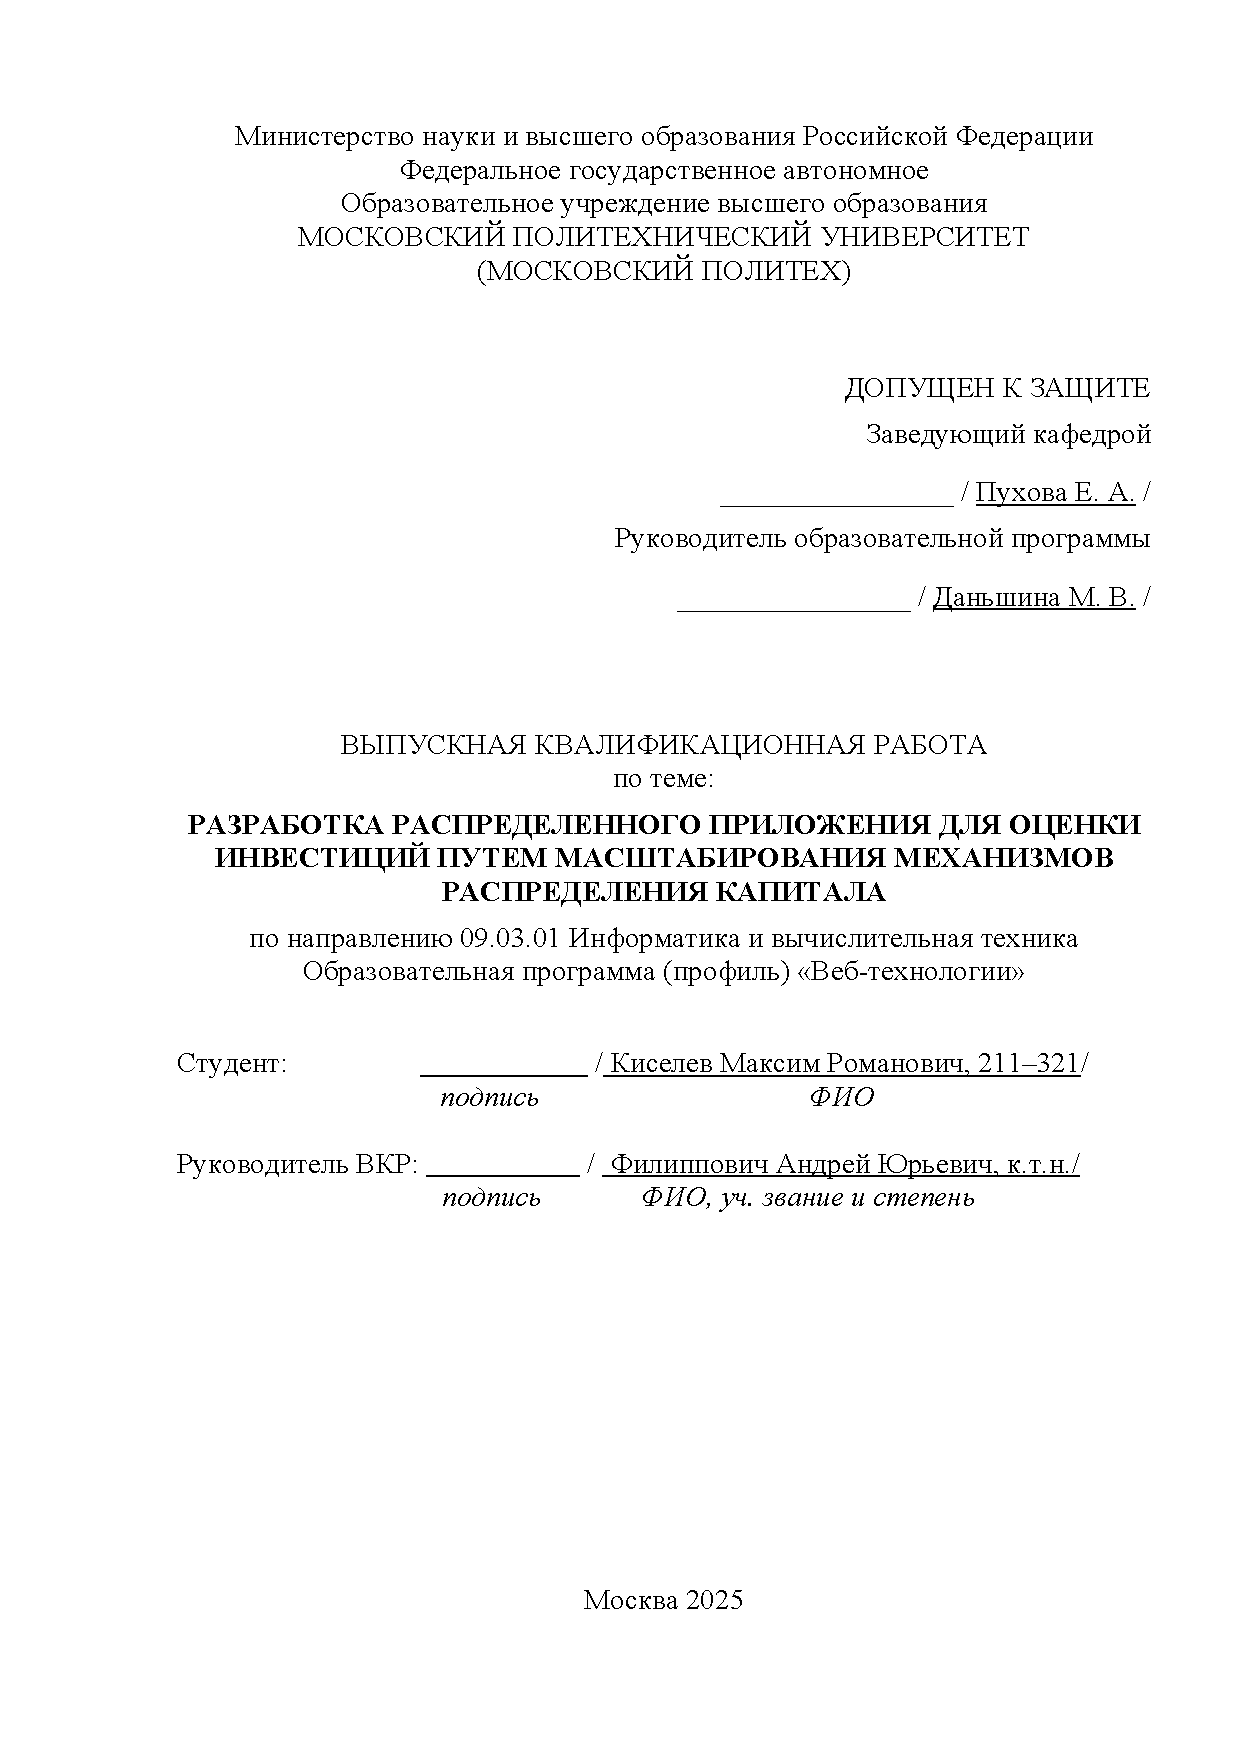
\includepdf[pages={1-5}]{./assets/TitlePage.pdf}

\renewcommand{\contentsname}{\centerline{СОДЕРЖАНИЕ}}
\setcounter{tocdepth}{1}
\tableofcontents

\newpage
\begin{center}
  \textbf{ВВЕДЕНИЕ}
\end{center}
\addcontentsline{toc}{chapter}{ВВЕДЕНИЕ}

Привлечение инвестиций на начальных этапах развития остается главным вызовом для многих компаний \cite{bernstein2017attracting}. Существующие механизмы финансирования ранних стадий обладают рядом фундаментальных ограничений, включая неравномерное распределение информации между участниками, субъективность при оценке проектов и недостаточную защиту интеллектуальной собственности. В результате формируются значительные препятствия, затрудняющие взаимодействие между инновационными предпринимателями и потенциальными инвесторами, заинтересованными в выявлении и развитии многообещающих проектов.


Актуальность данной работы обусловлена растущей потребностью в создании более справедливой и эффективной системы распределения ресурсов для инновационных проектов на ранних стадиях. Существующие механизмы инвестирования в значительной степени полагаются на субъективные факторы, такие как личность основателя, его социальные связи и престиж образовательных учреждений, которые он окончил, вместо объективной оценки потенциала самой идеи. Это приводит к неоптимальному распределению ресурсов, когда перспективные проекты остаются без финансирования, а менее инновационные, но лучше представленные или имеющие более сильные связи проекты привлекают непропорционально большие инвестиции.


Развитие современных технологий, в частности, блокчейна \cite{nakamoto2008bitcoin} и искусственного интеллекта, включая большие языковые модели \cite{vaswani2017attention},  открывает новые возможности для трансформации системы венчурного инвестирования. Блокчейн-технологии обеспечивают необходимую инфраструктуру для создания прозрачных, безопасных и неизменяемых записей о правах собственности, транзакциях и инвестиционных решениях. Криптографические протоколы, в частности, доказательства с нулевым разглашением (zero-knowledge proofs), позволяют верифицировать информацию без ее полного раскрытия, что критически важно для защиты интеллектуальной собственности.

Искусственный интеллект, в свою очередь, предоставляет инструменты для объективного анализа и оценки потенциала проектов на основе структурированных данных, исторических паттернов и рыночных трендов. Алгоритмические системы оценки могут минимизировать влияние личных предубеждений и субъективных факторов, обеспечивая более справедливое распределение капитала.

Интеграция механизмов квадратичного финансирования, разработанных группой исследователей в области криптоэкономики, и возрастающих кривых ограничения (augmented bonding curves) позволяет оптимизировать распределение ресурсов для инновационных проектов, учитывая не только размер инвестиций, но и широту поддержки в сообществе. Концепция механизма распределения ресурсов с балансом автоматизации и человеческого контроля обеспечивает баланс между эффективностью алгоритмической оценки и необходимостью человеческого контроля над принципиальными решениями.

Целью данной работы является масштабирование механизма слепого инвестирования в ранние стадии стартапов, основанного на блокчейн-технологиях и искусственном интеллекте, объективную оценку проектов и оптимальное распределение капитала на основе принципов квадратичного финансирования и возрастающих кривых ограничения.

Для достижения поставленной цели в работе решаются следующие задачи:
\begin{enumerate}
  \item Проведение анализа существующих механизмов инвестирования в ранние стадии, выявление их преимуществ и недостатков
  \item Изучение и адаптация механизмов квадратичного финансирования, возрастающих кривых ограничения и дистиллированного человеческого суждения
  \item Разработка архитектуры платформы, обеспечивающей защиту интеллектуальной собственности, объективную оценку и оптимальное распределение капитала
  \item Выбор и обоснование технологического стека для реализации платформы
  \item Разработка прототипа платформы с ключевыми механизмами и функциональностью
  \item Проведение экспериментальной оценки эффективности предложенной платформы
  \item Разработка рекомендаций по интеграции и масштабированию решения
\end{enumerate}

Предметом исследования являются механизмы распределения ресурсов и оценки инновационных проектов на ранних стадиях, основанные на технологиях блокчейн и искусственного интеллекта. Объектом исследования выступает процесс инвестирования в ранние стадии инновационных проектов.

Практическая значимость работы заключается в создании новой парадигмы инвестирования, которая позволит преодолеть структурные ограничения существующих механизмов и обеспечить более эффективное распределение капитала для инновационных проектов. Это может способствовать ускорению технологического развития, созданию новых рабочих мест и повышению глобальной конкурентоспособности экономики.

Заказчиками данного исследования выступают венчурные фонды, стремящиеся оптимизировать процессы скаутинга и предварительного отбора перспективных проектов, а также инновационные экосистемы, заинтересованные в создании более справедливой и эффективной системы распределения ресурсов для стартапов на ранних стадиях.

% Глава 1
\newpage
\begin{center}
  \textbf{1 АНАЛИТИЧЕСКИЙ ОБЗОР }
\end{center}
\refstepcounter{chapter}
\addcontentsline{toc}{chapter}{1 АНАЛИТИЧЕСКИЙ ОБЗОР }

\section{Анализ предметной области и проблематики}

Рынок инвестиций в ранние стадии стартапов представляет собой сложную и многогранную экосистему, в которой участвуют разнообразные субъекты – от основателей и индивидуальных инвесторов до венчурных фондов и корпоративных акселераторов. Такая экосистема характеризуется высокой степенью неопределенности и информационной асимметрией, что приводит к появлению структурных проблем, негативно влияющих на эффективность распределения ресурсов.

Одной из ключевых проблем является информационная асимметрия между основателями стартапов и потенциальными инвесторами. Основатели обладают глубоким пониманием своих проектов, однако при необходимости привлечения инвестиций вынуждены раскрывать конфиденциальную информацию, что создаёт риск утечки интеллектуальной собственности. В свою очередь, инвесторы ограничены в доступе к полной информации о проекте и его перспективах, что затрудняет объективную оценку и вынуждает опираться на косвенные сигналы, такие как образование и опыт основателей. Исследования подтверждают, что данная информационная асимметрия существенно влияет на эффективность распределения ресурсов: согласно данным CB Insights, около 38\% стартапов терпят неудачу из-за отсутствия финансирования, а многие перспективные проекты остаются без поддержки из-за неспособности адекватно донести свой потенциал до инвесторов. При этом инвесторы сталкиваются с феноменом «ложных позитивов», когда проекты, успешно привлекающие финансирование, впоследствии не оправдывают ожиданий, что приводит к неэффективному распределению капитала.

Вторая критическая проблема связана с субъективностью оценки и предвзятостью при принятии инвестиционных решений. Традиционные методы оценки стартапов на ранних стадиях во многом опираются на субъективные факторы, такие как личные качества основателя, его презентационные навыки, социальные связи и репутация. Исследования, проведённые Harvard Business Review, указывают на то, что инвесторы часто руководствуются эвристиками и интуитивными оценками, подверженными влиянию когнитивных предубеждений. Эмпирические данные демонстрируют наличие систематической предвзятости в отношении определённых групп основателей: согласно отчёту PitchBook, в 2020 году женщины-основатели получили лишь 2,3\% всего венчурного финансирования, несмотря на сопоставимые или даже более высокие показатели эффективности компаний, основанных женщинами. Аналогичные диспропорции наблюдаются и по отношению к представителям расовых и этнических меньшинств, а также основателям с нетрадиционным образовательным или профессиональным бэкграундом.

Третья важная проблема заключается в рисках для интеллектуальной собственности, возникающих в процессе привлечения инвестиций. Для получения финансирования основатели вынуждены раскрывать детали своих идей и технологий, что создаёт уязвимость перед кражей или копированием концепций, особенно если речь идёт о технологических стартапах, где ценность проекта определяется инновационными решениями. Традиционные механизмы защиты интеллектуальной собственности, такие как патенты и соглашения о неразглашении, зачастую оказываются неэффективными на ранних стадиях из-за высоких затрат, длительных процедур и проблем с их правоприменением. По данным Всемирной организации интеллектуальной собственности, процесс получения патента может затягиваться на срок от одного до трёх лет и требовать значительных финансовых вложений, что часто недоступно молодым стартапам.

Комплекс этих проблем создаёт существенные барьеры для эффективного функционирования рынка инвестиций в ранние стадии, приводя к неоптимальному распределению капитала, когда перспективные проекты остаются без необходимой поддержки, а проекты с меньшим потенциалом, но лучшей презентацией или более сильными социальными связями, получают непропорционально большие инвестиции, что в конечном итоге снижает эффективность инновационной экосистемы и замедляет технологический прогресс.

\section{Анализ целевой аудитории и её потребностей}

Целевая аудитория платформы слепого инвестирования охватывает три ключевые группы участников экосистемы ранних инвестиций: основателей стартапов, инвесторов ранних стадий и венчурные фонды. Каждая из этих групп характеризуется специфическими потребностями и сталкивается с уникальными вызовами, что должно быть учтено при разработке платформы.

Основатели стартапов и авторы инновационных идей, являющиеся первой группой, представляют предпринимателей на предпосевной и посевной стадиях, стремящихся привлечь финансирование для реализации своих идей. Они требуют, во-первых, обеспечения защиты интеллектуальной собственности при представлении идей потенциальным инвесторам, поскольку результаты опроса 500 основателей технологических стартапов свидетельствуют о том, что 73\% из них выражают обеспокоенность возможной кражей интеллектуальной собственности. Во-вторых, основатели нуждаются в доступе к капиталу, который должен основываться на объективной оценке потенциала идеи, а не на субъективных факторах, таких как опыт, образование или социальные связи, что подтверждается тем, что 82\% основателей считают, что их проекты отвергаются по причинам, не связанным с качеством самой идеи. Третьим требованием является получение конструктивной обратной связи для совершенствования идеи и бизнес-модели, так как около 65\% основателей отмечают, что отсутствие качественной обратной связи представляет существенное препятствие для развития их проектов. И, наконец, они стремятся минимизировать затраты времени и ресурсов на привлечение инвестиций, что особенно актуально, учитывая, что процесс привлечения посевного финансирования в среднем занимает от шести до девяти месяцев.

Вторую группу составляют инвесторы ранних стадий, для которых важным является обеспечение доступа к качественному потоку сделок с высоким потенциалом. Согласно данным Angel Capital Association, типичный инвестор рассматривает около 40 проектов для каждой инвестиции, что требует значительных временных затрат. Помимо этого, инвесторам необходимы объективные данные для оценки потенциала проектов в условиях ограниченного объёма информации; исследования показывают, что 78\% инвесторов ранних стадий указывают на недостаток объективных данных как основную проблему при оценке стартапов. Важным аспектом является также снижение транзакционных издержек, связанных с поиском, отбором и проведением due diligence, поскольку на каждую инвестицию инвестор затрачиваеют от 20 до 40 часов. Наконец, инвесторы стремятся к диверсификации инвестиционного портфеля, предпочитая инвестировать в 10–15 проектов, что позволяет распределить риски, несмотря на ограничения, связанные с оценкой большого количества проектов.

Третьей группой являются венчурные фонды и институциональные инвесторы, для которых ключевыми требованиями выступают наличие эффективных механизмов скаутинга и предварительного отбора перспективных проектов для последующих раундов инвестиций, при этом в среднем такие фонды рассматривают от 100 до 200 проектов для каждой инвестиции. Помимо этого, они нуждаются в аналитических инструментах для объективной оценки потенциала стартапов на ранних стадиях, поскольку исследования Cambridge Associates показывают, что фонды, применяющие структурированные аналитические подходы, достигают более высокой доходности, чем те, кто опирается преимущественно на интуитивные оценки. Не менее важна и возможность отслеживания рыночных трендов и выявления перспективных направлений на ранних этапах развития, о чем свидетельствуют данные, согласно которым около 65\% венчурных фондов отмечают существенные трудности в данной области. Кроме того, значительное внимание уделяется снижению временных и ресурсных затрат на первичный скрининг проектов, поскольку этот этап требует значительных усилий, а большинство рассматриваемых проектов отклоняется на ранних стадиях.

Проведённый анализ целевой аудитории демонстрирует, что, несмотря на различия в потребностях, все три группы заинтересованы в создании более эффективной, объективной и прозрачной системы оценки и финансирования инновационных проектов на ранних стадиях. Основатели стремятся к защите своих идей и объективной оценке их потенциала, инвесторы ранних стадий нуждаются в качественном потоке сделок и объективных данных для принятия решений, а венчурные фонды ориентированы на эффективные механизмы скаутинга и предварительного отбора проектов. Таким образом, платформа слепого инвестирования, основанная на блокчейн-технологиях и искусственном интеллекте, имеет потенциал для удовлетворения указанных потребностей через обеспечение защиты интеллектуальной собственности, объективной оценки проектов и оптимального распределения ресурсов.

\section{Обзор существующих решений и их ограничений}

В современной экосистеме инвестирования применяются различные подходы, каждый из которых частично решает обозначенные проблемы, но не способен обеспечить комплексную защиту интеллектуальной собственности, объективную оценку проектов и оптимальное распределение капитала одновременно.

Традиционные венчурные фонды и инвесторы представляют собой наиболее распространённый механизм финансирования ранних стадий, основанный на личных встречах, презентациях и субъективной оценке потенциала проектов и команд. Преимущества данного подхода заключаются в наличии доступа к экспертной поддержке и менторству, возможности установления долгосрочных отношений между основателями и инвесторами, гибкости в структурировании сделок и условия инвестирования, а также наличии широкой сети контактов, которую инвесторы могут предоставить. Однако существенные ограничения этого механизма проявляются в высокой степени субъективности и предвзятости при оценке проектов, что подтверждают исследования Гарвардской бизнес-школы, указывающие на двойное предпочтение инвестиций в основателей определённого пола и расы при прочих равных условиях. Дополнительно, зависимость от социальных связей и репутации, о чём свидетельствуют данные Stanford Graduate School of Business (более 70\% успешных сделок проходят через личные рекомендации), а также необходимость полного раскрытия идеи, создающая риск для интеллектуальной собственности (62\% основателей, согласно опросу National Venture Capital Association, обеспокоены вопросами конфиденциальности), и географическая концентрация венчурных инвестиций, ограничивающая доступ к капиталу для основателей из других регионов, существенно снижают эффективность данного подхода.

Альтернативными механизмами являются платформы краудфандинга и токенизированные системы финансирования, которые способствуют демократизации доступа к капиталу, позволяя привлекать финансирование без зависимости от традиционных связей, а также обеспечивают рыночную валидацию идеи через прямой отклик потенциальных пользователей. Такие подходы также способствуют созданию сообщества вокруг проекта на ранних стадиях и обладают высокой ликвидностью в случае токенизированных систем. С другой стороны, они требуют публичного раскрытия идеи в деталях, что не решает проблему защиты интеллектуальной собственности, ориентированы преимущественно на проекты с прямой потребительской привлекательностью (ограничивая возможности для B2B и инфраструктурных решений), и часто решения о финансировании принимаются непрофессиональной аудиторией, что может приводить к поддержке коммерчески нежизнеспособных проектов. Кроме того, высокие маркетинговые затраты и регуляторные риски, особенно в случае токенизированных систем, также являются значительными ограничениями.

Акселераторы, инкубаторы и алгоритмические платформы инвестиций, такие как Y Combinator, Techstars, AngelList и Republic, предлагают структурированные программы поддержки стартапов, объединяющие менторство, образовательные компоненты и доступ к инвесторам. Структурированный процесс отбора и поддержки проектов создаёт чёткие рамки для развития, что особенно важно для неопытных основателей \cite{thiel2014zero}, а доступ к обширным сетям контактов и экспертизе ускоряет валидацию идей и выход на рынок. При этом частичная автоматизация инвестиционных процессов снижает транзакционные издержки, а стандартизация документации упрощает юридические аспекты финансирования. Однако и эти механизмы не лишены существенных ограничений. Во-первых, процесс отбора остаётся субъективным и подверженным предубеждениям, что подтверждают исследования MIT, демонстрирующие влияние демографических характеристик основателей на решения акселераторов. Во-вторых, требование полного раскрытия деталей идеи сохраняется, что не устраняет проблемы защиты интеллектуальной собственности. В-третьих, высокая конкуренция за места в ведущих программах (например, Y Combinator принимает менее 3\% заявителей) значительно снижает шансы на участие, а экономические трудности, связанные с передачей значительной доли в проекте (обычно 6–10\%), могут не соответствовать ценности на поздних стадиях. Наконец, географические ограничения продолжают оставаться барьером для основателей, расположенных вне основных инновационных хабов.

Сравнительный анализ эффективности существующих подходов показывает, что ни один из них не способен обеспечить одновременно надёжную защиту интеллектуальной собственности, объективную оценку проектов и оптимальное распределение капитала. Традиционные венчурные фонды и акселераторы предлагают качественную экспертную оценку, но страдают от субъективности и предвзятости, тогда как платформы краудфандинга отличаются доступностью для различных категорий основателей, но менее эффективны с точки зрения долгосрочной коммерческой оценки. Эффективность распределения ресурсов, измеряемая отношением числа успешных проектов к общему числу профинансированных, остаётся низкой – по данным CB Insights, около 75\% венчурных инвестиций не оправдывают ожиданий, что свидетельствует о системных недостатках существующих механизмов.

Таким образом, анализ существующих решений указывает на необходимость создания комплексного механизма, который бы одновременно обеспечивал защиту интеллектуальной собственности, объективную оценку проектов и оптимальное распределение капитала с учётом как объёма инвестиций, так и широты поддержки в инновационном сообществе. Платформа слепого инвестирования, основанная на блокчейн-технологиях, искусственном интеллекте и механизмах квадратичного финансирования, обладает потенциалом для удовлетворения этих требований и формирования более эффективной и справедливой экосистемы для инноваций.

\section{Технологический обзор}

Разработка платформы слепого инвестирования предполагает интеграцию передовых технологий, таких как блокчейн, искусственный интеллект, криптографические методы защиты интеллектуальной собственности и системы токенизации.

\subsection{Блокчейн-технологии в контексте финансирования инноваций}

При реализации механизмов слепого инвестирования могут быть использованы различные типы блокчейн-платформ. Так, публичные блокчейны (например, Ethereum, Solana, Polkadot) обеспечивают максимальную прозрачность и децентрализацию \cite{antonopoulos2018ethereum}, хотя сталкиваются с ограничениями по масштабируемости и стоимости транзакций. Приватные и консорциумные блокчейны, такие как Hyperledger Fabric и Corda, позволяют достичь более высокой производительности и контроля над доступом, но при этом ограничивают степень децентрализации. Дополнительно решения второго уровня (Layer 2), такие как Optimism, Arbitrum и zkSync, предоставляют возможности масштабирования на основе публичных блокчейнов, сохраняя их ключевые преимущества.

Особый интерес для реализации платформы представляют возможности, которые предоставляет блокчейн-технология. Так, смарт-контракты, являющиеся самоисполняющимися программными протоколами, позволяют автоматизировать процессы инвестирования, распределения средств и управления правами собственности \cite{antonopoulos2018ethereum}. Токенизация активов, то есть представление прав собственности, доступа или участия в цифровом виде, способствует дроблению инвестиций, обеспечивает их ликвидность и открывает новые возможности для инвестирования \cite{dixon2018crypto}. Кроме того, криптографические методы, такие как доказательства с нулевым разглашением \cite{ben2014succinct}, позволяют подтвердить владение идеей без раскрытия избыточной информации, что крайне важно для защиты интеллектуальной собственности. Наконец, децентрализованные автономные организации (DAO), управляемые через смарт-контракты и коллективное принятие решений, обеспечивают децентрализованное управление платформой и распределение средств на основе установленных правил.

\subsection{Искусственный интеллект и его применение для оценки потенциала проектов}

Для оценки потенциала инновационных проектов применимы различные алгоритмы и модели искусственного интеллекта. Так, модели машинного обучения (например, Random Forests, Gradient Boosting, нейронные сети) могут обучаться на исторических данных о стартапах для прогнозирования вероятности успеха, выявляя скрытые зависимости и паттерны. Технологии обработки естественного языка (NLP) позволяют анализировать текстовые описания проектов, выделяя ключевые концепции и оценивая их оригинальность, при этом современные модели, такие как BERT и GPT, обеспечивают глубокое понимание контекста. Анализ рыночных данных с помощью алгоритмов искусственного интеллекта помогает оценить потенциальный размер рынка, уровень конкуренции и оптимальные временные рамки для выхода на рынок, что имеет решающее значение для оценки коммерческого потенциала. Наконец, ансамблевые методы, объединяющие несколько алгоритмов и источников данных, способствуют получению более надёжных и объективных оценок, снижая влияние случайного шума и предвзятости отдельных моделей.

Интеграция искусственного интеллекта в платформу слепого инвестирования позволяет реализовать ряд функций, включая ранжирование проектов по потенциальной доходности и вероятности успеха, выявление инновационных и оригинальных идей среди множества схожих предложений, определение оптимального размера инвестиций и временного горизонта для различных типов проектов, а также предоставление объективной обратной связи основателям для совершенствования их бизнес-моделей и идентификацию потенциальных синергий между проектами и инвесторами.

\subsection{Криптографические механизмы защиты интеллектуальной собственности}

В условиях необходимости защиты интеллектуальной собственности при представлении инновационных идей инвесторам целесообразно применять современные криптографические механизмы. В числе наиболее перспективных методов выделяются доказательства с нулевым разглашением \cite{ben2014succinct}, позволяющие доказать истинность утверждения без раскрытия избыточной информации, а также временное закрепление данных на блокчейне, создающее неизменяемое доказательство существования информации в определённый момент времени \cite{benet2014ipfs}. Гомоморфное шифрование даёт возможность проводить вычисления над зашифрованными данными без предварительного расшифрования, а протоколы мультисторонних вычислений (MPC) позволяют нескольким сторонам совместно вычислять функцию, не раскрывая при этом свои исходные данные. Важным является и механизм контролируемого раскрытия информации, который позволяет регулировать объём и характер предоставляемых данных в зависимости от этапа инвестиционного процесса и уровня доверия между участниками.

Интеграция указанных криптографических методов позволяет создать многоуровневую систему защиты: на начальном этапе основатели могут представить общую концепцию и метаданные проекта (такие как отрасль, целевой рынок, ожидаемая доходность) с одновременным шифрованием деталей реализации; затем алгоритмы искусственного интеллекта проводят оценку на основе этих метаданных с применением гомоморфного шифрования; после принятия решения о финансировании и подписания юридически обязывающих соглашений происходит контролируемое раскрытие деталей проекта.

\subsection{Токенизация и механизмы рыночного ценообразования в цифровой экономике}

Токенизация, представляющая собой процесс преобразования прав на актив в цифровой токен, открывает новые возможности для фрагментации инвестиций, обеспечения ликвидности и создания эффективных механизмов ценообразования \cite{cong2020tokenomics}. При этом могут использоваться различные модели токенизации. Так, токены собственности представляют долю в проекте и дают право на получение дивидендов или участие в управлении, подобно традиционным акциям, но с большей ликвидностью; токены доходности позволяют получать долю от доходов или прибыли проекта без предоставления прав собственности; утилитарные токены обеспечивают доступ к продуктам или услугам, разрабатываемым проектом, и могут использоваться для их предварительной продажи \cite{catalini2018initial}; гибридные токены, в свою очередь, сочетают характеристики нескольких типов токенов для создания более гибких инвестиционных инструментов.

Для определения цены токенов и обеспечения эффективного рыночного ценообразования применяются различные механизмы. Среди них автоматические маркет-мейкеры представляют собой алгоритмические протоколы, обеспечивающие ликвидность и ценообразование без использования централизованной книги заказов, как это реализовано, например, в Uniswap, Balancer и Curve. Аукционные механизмы, основанные на конкурентной борьбе между участниками, включают форматы, такие как английский, голландский и Викри, каждый из которых обладает своими характеристиками с точки зрения эффективности и устойчивости к манипуляциям. Дополнительно используются кривые ограничения, представляющие математические функции, определяющие цену токена в зависимости от его предложения, что позволяет создать предсказуемый механизм ценообразования, адаптируемый к различным целям.

Особое внимание в рамках платформы слепого инвестирования уделяется возрастающим кривым ограничения (BC), которые обеспечивают предсказуемый механизм ценообразования, основанный на принципах спроса и предложения, автоматическое создание ликвидности для токенов проектов и возможность распределения части средств на развитие проекта посредством резервных пулов.

% Глава 2
\newpage
\begin{center}
  \textbf{2. ТЕОРЕТИЧЕСКИЕ ОСНОВЫ МЕХАНИЗМОВ РАСПРЕДЕЛЕНИЯ РЕСУРСОВ}
  \end{center}
  \refstepcounter{chapter}
  \addcontentsline{toc}{chapter}{2. ТЕОРЕТИЧЕСКИЕ ОСНОВЫ МЕХАНИЗМОВ распределения ресурсов}

  \section{Квадратичное финансирование как механизм оптимального распределения ресурсов}

  Квадратичное финансирование (Quadratic Funding, QF) представляет собой математически обоснованный механизм поддержки общественных благ, разработанный группой исследователей экономической теории, который изложен в работе «Либеральный радикализм: формальные правила для общества, нейтрального к процветанию и политическому голосу» (2019). Механизм основывается на теоретических положениях экономической теории общественных благ, характеризующихся неисключаемостью и неконкурентностью, что особенно актуально для инновационных проектов на ранних этапах развития, обладающих признаками частичных общественных благ вследствие создания положительных внешних эффектов для всей экосистемы. Традиционные рыночные механизмы зачастую оказываются неэффективными в решении проблемы «безбилетника», когда отдельные участники могут извлекать выгоду без фактического участия в финансировании. В этой связи квадратичное финансирование представляет собой инновационный метод, позволяющий агрегировать индивидуальные предпочтения участников и распределять ресурсы с учётом коллективной полезности.

  В основе данного механизма лежит принцип, согласно которому размер софинансирования из общего пула определяется не только суммой индивидуальных вкладов, но и числом участников, что позволяет учитывать широту поддержки проекта. Иными словами, подход предполагает, что проекты, пользующиеся поддержкой большого количества участников, даже при наличии сравнительно небольших индивидуальных вкладов, получают преимущество в виде увеличенного размера софинансирования по сравнению с проектами, финансируемыми за счёт нескольких крупных инвестиций. Такой принцип нелинейного увеличения софинансирования отражает возрастание общественной ценности проектов, имеющих широкий круг сторонников, и одновременно стимулирует участников раскрывать свои истинные предпочтения без склонности к стратегическим манипуляциям.

  \subsection{Теоретические основы квадратичного финансирования}

  Математическое обоснование механизма квадратичного финансирования строится на предпосылках теории общественных благ и механизмов выявления индивидуальных предпочтений. Пусть имеется $n$ проектов и $m$ участников, при этом каждый участник $i$ вносит вклад $c_{ij}$ в проект $j$. Общий вклад проекта определяется как
  \[
    C_j = \sum_{i=1}^{m} c_{ij}.
  \]
  Согласно принципам квадратичного финансирования, размер софинансирования из общего пула $M$ для проекта $j$ определяется по формуле
  \[
    M_j = \alpha \left( \sqrt{\sum_{i=1}^{m} c_{ij}} \right)^2 - \sum_{i=1}^{m} c_{ij},
  \]
  где $\alpha$ является нормирующим множителем, обеспечивающим распределение всего пула. Таким образом, итоговое финансирование проекта представляется суммой его прямых вкладов и софинансирования:
  \[
    F_j = \sum_{i=1}^{m} c_{ij} + M_j.
  \]
  Данный подход обеспечивает создание системы, в которой проекты, поддержанные широким кругом участников посредством множества небольших вкладов, получают более значительное дополнительное финансирование по сравнению с проектами, для которых суммарный вклад исходит от ограниченного числа крупных инвесторов. Кроме того, механизм характеризуется нелинейным ростом софинансирования с увеличением числа участников, что непосредственно отражает возрастание общественной ценности поддерживаемых проектов. Такой принцип работы способствует формированию стимулов для участников системы, побуждая их выражать истинные предпочтения и минимизируя вероятность стратегического искаженного голосования.

  \subsection{Математическая модель квадратичного финансирования}

  Математическая модель, описывающая механизм квадратичного финансирования, опирается на вышеуказанные соотношения и демонстрирует, каким образом распределяются ресурсы между проектами. В этой модели суммарный вклад каждого проекта определяется суммой индивидуальных инвестиций, а затем к этой сумме прибавляется дополнительное финансирование, вычисляемое с использованием квадратного корня от общего вклада. Такой подход приводит к тому, что проекты с широкой поддержкой получают относительно больше дополнительных средств, что отражает их высокую общественную значимость. При этом механизм учитывает нелинейный эффект от увеличения числа участников, что позволяет эффективно дифференцировать проекты по степени общественной востребованности и минимизировать возможности манипуляций со стороны крупных инвесторов.

  \subsection{Преимущества и ограничения квадратичного финансирования}

  Преимущества квадратичного финансирования заключаются в том, что данный механизм теоретически обеспечивает оптимальное распределение ресурсов для максимизации общественной полезности, поскольку учитывает как суммарный объём инвестиций, так и число участников, поддерживающих проект. Это приводит к демократизации процесса принятия инвестиционных решений, поскольку не доминируют крупные инвесторы, а также позволяет выявлять истинные предпочтения участников, что дополнительно усиливает эффективность распределения ресурсов. Кроме того, механизм оказывается особенно полезным для поддержки инновационных проектов, способных создавать значительные положительные внешние эффекты для всей экосистемы.

  Однако, наряду с указанными преимуществами, квадратичное финансирование имеет и ряд ограничений, которые необходимо учитывать при разработке и внедрении платформ. Среди таких ограничений можно отметить уязвимость системы к атакам Сибиллы, когда фиктивное создание множественных аккаунтов может привести к искусственному увеличению вклада в проект, а также зависимость эффективности механизма от наличия достаточного и устойчивого внешнего пула финансирования. Дополнительной проблемой является относительная сложность механизма для конечных пользователей, что требует разработки образовательных программ и упрощённых интерфейсов для облегчения его восприятия. Наконец, теоретически оптимальный механизм может оказаться слишком сложным для практической реализации, что влечёт за собой необходимость поиска компромиссов между математической строгостью и удобством применения.

  \section{Возрастающие кривые ограничения для токенизации проектов}

  Возрастающие кривые ограничения (Augmented Bonding Curves, ABC) представляют собой механизм, направленный на токенизацию и финансирование проектов, который позволяет создать предсказуемую модель ценообразования и ликвидности для токенов на ранних стадиях развития. Практическое применение данной концепции наблюдается в современных платформах финансирования, таких как Allo Capital \cite{allo_capital}, где механизмы кривых ограничения интегрированы с другими инструментами поддержки общественных благ. В основе подхода лежит использование математической функции, определяющей цену токена в зависимости от его предложения, что позволяет участникам получать токены проекта посредством «связывания» базового актива (например, ETH) с определённой кривой, а при последующем их возврате — получать базовый актив по цене, заданной данной функцией.

  Наиболее распространёнными формами представления функции ценообразования являются линейная, квадратичная и экспоненциальная модели, которые описываются, соответственно, выражениями $P(S) = mS + b$, $P(S) = aS^2 + bS + c$ и $P(S) = e^{kS}$. Каждая из этих моделей обладает своими особенностями, однако общим для всех является зависимость цены токена от текущего предложения. Возрастающие кривые ограничения совершенствуют базовую концепцию за счёт интеграции дополнительных механизмов. Среди них особое место занимает формирование резервного пула, куда направляется часть средств, полученных от продажи токенов, что способствует поддержанию ликвидности и финансированию развития проекта. Помимо этого, на начальном этапе проекта вводится специальная фаза разработки, в течение которой токены могут быть приобретены, но не проданы, что обеспечивает стабильное финансирование и защищает от спекулятивных атак. Механизмы стабилизации реализуются через введение дополнительных правил и ограничений, направленных на снижение волатильности, а также посредством применения инструментов вестинга и блокировки, позволяющих ограничить возможность продажи токенов в определённые периоды и тем самым предотвратить резкие изменения ликвидности и цен.

  \subsection{Принципы работы возрастающих кривых ограничения}

  Базовая идея кривой ограничения заключается в том, что цена токена определяется функцией $P(S)$, где $P$ означает цену, а $S$ --- текущее предложение токенов. В данном контексте используются различные формы функции, каждая из которых отражает особенности процесса ценообразования в зависимости от специфики проекта. Математическая модель позволяет участникам покупать токены, что сопровождается «связыванием» базового актива с кривой, а последующая продажа токенов осуществляется с возвратом базового актива по цене, определяемой данной функцией.

  \subsection{Токенизация проектов и формирование ценности}

  При использовании возрастающих кривых ограничения каждый проект, представленный на платформе, получает свою токенизированную репрезентацию, параметры которой устанавливаются на основе специфических характеристик, таких как отрасль, стадия развития и потенциальный рынок. В этом случае инвесторы приобретают токены через соответствующую кривую ограничения, при этом значительная часть полученных средств, условно составляющая около 70\%, направляется в резервный пул для финансирования дальнейшего развития проекта, а оставшаяся часть, например 30\%, используется для обеспечения ликвидности через резерв кривой. По мере развития проекта и роста спроса на его токены их цена повышается в соответствии с установленной кривой, что отражает рыночную оценку потенциала проекта. Инвесторы, в свою очередь, после завершения начальной фазы разработки получают возможность продать токены обратно через кривую, получая базовый актив по текущей цене.

  \subsection{Механизмы стабилизации и обеспечения ликвидности}

  Для поддержания стабильности и ликвидности токенизированных проектов в рамках платформы слепого инвестирования применяется совокупность мер, направленных на снижение рисков спекулятивных атак и резких ценовых колебаний. В частности, на начальном этапе проекта вводится фаза разработки, в ходе которой токены могут быть приобретены, но не проданы, что обеспечивает стабильное финансирование на ранних стадиях и минимизирует вероятность манипуляций. Дополнительно внедряются ограничения на объем транзакций, устанавливающие максимальный размер покупки или продажи в рамках одной сделки, что способствует снижению риска резких изменений цены. Значительную роль играют временные замки, ограничивающие возможность продажи токенов в определённые периоды, что особенно важно для защиты интересов ранних инвесторов и членов команды проекта. Механизмы динамических комиссий, при которых размер комиссионных увеличивается в периоды высокой волатильности или при больших объемах торгов, также способствуют дестимулированию спекулятивного поведения. Наконец, автоматическое перебалансирование резервов позволяет корректировать распределение средств между резервным пулом и резервом кривой в зависимости от рыночных условий и стадии развития проекта, что обеспечивает устойчивость системы.

  \subsection{Интеграция с системами распределения ресурсов}

  Интеграция возрастающих кривых ограничения с механизмами распределения ресурсов представляет собой важное звено в создании эффективной системы поддержки инновационных проектов. В данном случае проекты получают возможность финансирования не только через прямые инвестиции, осуществляемые посредством кривых ограничения, но и через софинансирование из общего пула, реализуемого с помощью квадратичного финансирования. При этом вклад, осуществляемый в рамках квадратичного финансирования, может корректироваться с учётом репутации инвесторов и их предыдущего опыта, что позволяет повысить эффективность распределения ресурсов. Размер пула для квадратичного финансирования динамически определяется пропорционально общему объему средств, привлечённых через кривые ограничения, что способствует формированию само масштабируемой экосистемы. Важным элементом данной интеграции является участие децентрализованных автономных организаций (DAO), посредством которых осуществляется управление параметрами кривых ограничения и распределением средств из общего пула, предоставляя держателям токенов платформы возможность влиять на ключевые решения.

  \section{Механизм распределения ресурсов с балансом автоматизации и человеческого контроля}

  Данный механизм представляет собой подход к интеграции искусственного интеллекта в процессы принятия решений и распределения ресурсов, при котором вычислительные алгоритмы выполняют основную работу по обработке данных, а конечное управление и определение стратегических направлений остаются за людьми. Такой баланс позволяет использовать вычислительные мощности для обработки больших объёмов информации, одновременно обеспечивая контроль над ключевыми параметрами системы со стороны экспертов и инвесторов.

  \subsection{Основополагающая идея механизма распределения ресурсов с балансом автоматизации и человеческого контроля}

  Основополагающая идея механизма распределения ресурсов с балансом автоматизации и человеческого контроля заключается в оптимальном распределении ролей между искусственным интеллектом и человеком, где алгоритмы выполняют функции первичной обработки и анализа больших массивов данных, выявления скрытых паттернов и зависимости, а также обеспечивают систематическую, непредвзятую оценку проектов с высокой масштабируемостью. В то же время человеческий фактор остаётся критически важным для определения высокоуровневых целей и ценностей системы, контроля за этичностью и корректностью алгоритмических решений, а также для вмешательства в ситуациях, требующих творческого подхода и нестандартного мышления. Такой синергичный подход позволяет эффективно сочетать вычислительные возможности современных алгоритмов с интуицией и экспертными знаниями, что особенно важно для систем, где финансовые решения должны быть сбалансированы с долгосрочными общественными интересами.

  \subsection{Практическое применение механизма распределения ресурсов с балансом автоматизации и человеческого контроля на платформе слепого инвестирования}

  Практическая реализация механизма распределения ресурсов с балансом автоматизации и человеческого контроля на платформе слепого инвестирования осуществляется на нескольких взаимосвязанных уровнях. На уровне оценки проектов искусственный интеллект проводит детальный анализ описаний проектов, рыночных данных и технических характеристик, формируя комплексную, многомерную оценку их потенциала. При этом инвесторы и эксперты играют важную роль в определении относительной значимости различных аспектов, устанавливая высокоуровневые критерии, а результаты анализа представляются в форме, способствующей принятию информированных инвестиционных решений. На уровне распределения ресурсов алгоритмы рассчитывают оптимальное распределение средств из общего пула, используя данные об индивидуальных вкладах, экспертных оценках и исторических тенденциях, при этом сообщество пользователей периодически участвует в голосовании по изменению параметров распределения, таких как вес различных факторов и доля средств для отдельных категорий проектов, а смарт-контракты автоматически исполняют распределительные решения в соответствии с установленными правилами. Управление платформой осуществляется посредством интеграции алгоритмов мониторинга, способных выявлять аномалии и потенциальные злоупотребления, с децентрализованной автономной организацией (DAO), которая принимает стратегические решения о развитии платформы и изменении регламентов, при этом мультисигнатурные механизмы обеспечивают согласование критически важных изменений между многочисленными независимыми участниками. На уровне защиты интеллектуальной собственности применяются криптографические протоколы, позволяющие автоматически защищать конфиденциальную информацию и предоставлять искусственному интеллекту возможность анализа данных без полного доступа к их содержанию, в то время как вопросы раскрытия информации регулируются экспертами, а система репутации стимулирует участников соблюдать высокие стандарты конфиденциальности.

  В результате комплексное применение механизма распределения ресурсов с балансом автоматизации и человеческого контроля позволяет создать систему, в которой технологическая эффективность и масштабируемость алгоритмов искусственного интеллекта гармонично сочетаются с человеческой мудростью, этическим суждением и стратегическим контролем, что имеет решающее значение для устойчивого распределения ресурсов и поддержки инноваций в долгосрочной перспективе.

  \section{UML-модель механизма распределения ресурсов}

  Для более наглядного представления механизма распределения ресурсов с балансом автоматизации и человеческого контроля была разработана UML-диаграмма вариантов использования (use case diagram), представленная на рисунке \ref{fig:uml-use-case-diagram}. Данная диаграмма демонстрирует взаимодействие различных акторов системы и распределение ролей между алгоритмическими и человеческими компонентами.

  \begin{figure}[h]
    \centering
    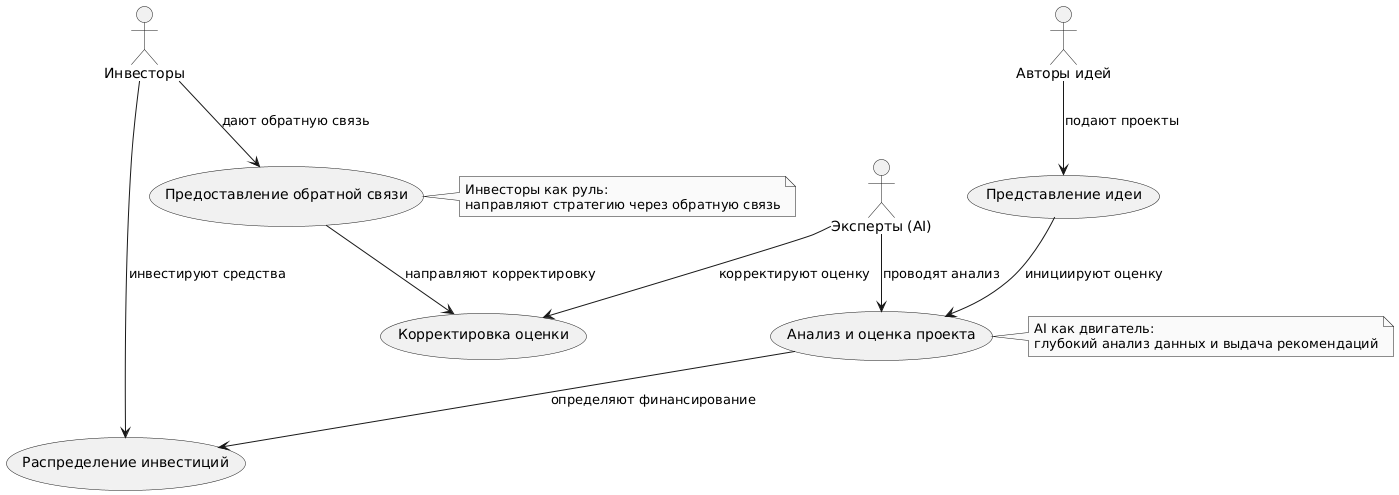
\includegraphics[width=0.9\textwidth]{./assets/uml-use-case-diagram.png}
    \caption{UML-диаграмма вариантов использования механизма распределения ресурсов с балансом автоматизации и человеческого контроля}
    \label{fig:uml-use-case-diagram}
  \end{figure}

  Как видно из диаграммы, в системе выделяются три основных группы участников: инвесторы, авторы идей и эксперты (представленные, в том числе, системами ИИ). Инвесторы участвуют в процессе предоставления обратной связи и непосредственного инвестирования средств, что направляет стратегию распределения ресурсов. Авторы идей подают свои проекты на рассмотрение через механизм представления идеи. Эксперты, включая аналитические системы на основе ИИ, выполняют ключевую роль по анализу и оценке проектов, а также корректировке предварительных оценок.

  Центральными процессами в системе являются:

  \begin{enumerate}
    \item Представление идеи -- процесс, при котором авторы формулируют и загружают свои проекты в систему с защитой интеллектуальной собственности.

    \item Анализ и оценка проекта -- основная аналитическая работа по многомерной оценке потенциала проекта, выполняемая в значительной степени автоматизированными системами с глубоким анализом данных.

    \item Предоставление обратной связи -- процесс, в котором инвесторы выражают свои предпочтения и видение направления развития.

    \item Корректировка оценки -- механизм коррекции и уточнения, где эксперты и инвесторы могут скорректировать предварительные результаты анализа.

    \item Распределение инвестиций -- финальный этап, на котором средства распределяются между проектами на основе комплексной оценки, полученной в результате работы механизма.
  \end{enumerate}

  Особенно важно отметить, что механизм построен по принципу, где алгоритмические компоненты выполняют основную вычислительную работу по обработке больших объемов данных, а человеческие компоненты направляют стратегию через обратную связь, определяют стратегические приоритеты и осуществляют контроль. Такой подход обеспечивает баланс эффективности и надежности, сочетая вычислительную мощь алгоритмов с ценностями и экспертизой человеческих участников.

  Данный механизм реализует принцип коллективного принятия решений, где автоматизация используется для обеспечения объективности и масштабируемости, а человеческое участие – для стратегического управления процессом и сохранения этических аспектов распределения ресурсов.

  % Глава 3
  \newpage
  \begin{center}
  \textbf{3. МАШТАБИРОВАНИЕ МЕХАНИЗМА ИНВЕСТИРОВАНИЯ}
\end{center}
\refstepcounter{chapter}
\addcontentsline{toc}{chapter}{3. МАШТАБИРОВАНИЕ МЕХАНИЗМА ИНВЕСТИРОВАНИЯ}

\section{Архитектура платформы и основные компоненты}

Архитектура платформы слепого инвестирования разработана с учётом принципов децентрализации, безопасности, масштабируемости и интероперабельности, что позволило интегрировать технологии блокчейна, искусственного интеллекта и современные криптографические механизмы в единую систему, способную обеспечить эффективное и справедливое распределение капитала для финансирования инновационных проектов. Данная архитектура построена на модульном принципе, когда различные компоненты, оставаясь взаимосвязанными, функционируют независимо, что обеспечивает гибкость системы и возможность эволюционного развития отдельных её частей. В основе проектирования лежит идея распределения критически важных данных и сервисов по сети, что устраняет единую точку отказа и позволяет обеспечить устойчивость к цензуре, а также применение криптографических методов и принципа минимального необходимого доступа, что гарантирует безопасность и защиту конфиденциальной информации. Кроме того, система сконструирована таким образом, чтобы сохранять высокую производительность при увеличении количества обрабатываемых проектов и пользователей, что достигается за счёт применения решений второго уровня для блокчейна и распределённых вычислений для реализации алгоритмов искусственного интеллекта. Применение открытых стандартов и протоколов способствует созданию интероперабельной среды, а механизмы коллективного управления обеспечивают адаптивность архитектуры к изменяющимся требованиям.

Базовый уровень архитектуры включает слой блокчейна, отвечающий за запись и верификацию транзакций, исполнение смарт-контрактов и токенизацию активов, а также протокольный слой, в котором реализуются специализированные алгоритмы защиты интеллектуальной собственности, квадратичного финансирования и возрастающих кривых ограничения. Дополнительные слои отвечают за аналитику и обработку данных с использованием искусственного интеллекта, а также за предоставление удобного пользовательского интерфейса, что позволяет участникам системы взаимодействовать с платформой на различных уровнях доступа. При этом интеграция с внешними системами, базами данных и другими блокчейн-платформами расширяет функциональные возможности всей системы.

Ключевые компоненты системы охватывают комплексное управление проектами, инвестиционный механизм, аналитический движок, систему защиты интеллектуальной собственности, платформу децентрализованного управления, а также интерфейсы и API для взаимодействия с внешними сервисами. Функциональность управления проектами реализуется посредством представления и категоризации идей, сопровождаемой механизмами проверки качества и верификации данных, что обеспечивает конфиденциальное взаимодействие между основателями и инвесторами. Инвестиционный механизм базируется на математически обоснованных схемах токенизации и распределения ресурсов, позволяющих оптимизировать финансирование посредством квадратичного механизма и защиты от атак, включая атаки Сибиллы, посредством специально разработанных смарт-контрактов. Аналитический движок, построенный на современных моделях искусственного интеллекта, позволяет проводить комплексный анализ потенциала проектов, оценивать рыночные тренды, выявлять закономерности и прогнозировать успешность проектов. В свою очередь, система защиты интеллектуальной собственности включает в себя современные криптографические протоколы, такие как доказательства с нулевым разглашением, а также механизмы временного закрепления информации на блокчейне и безопасной многосторонней вычислимости. Организация децентрализованного управления посредством DAO, поддерживаемая механизмами голосования и системы репутации, позволяет обеспечить прозрачное и гибкое управление платформой, а разработанные интерфейсы и API делают систему доступной для широкого круга пользователей.

При выборе стека технологий основное внимание уделялось использованию EVM-совместимых блокчейнов для реализации смарт-контрактов, а также решений второго уровня, способствующих повышению масштабируемости и снижению транзакционных издержек. В качестве языков программирования для смарт-контрактов применялись Solidity и Vyper, а разработка сопровождалась использованием проверенных фреймворков, таких как Hardhat и OpenZeppelin. Современные криптографические методы, включая zk-SNARKs и zk-STARKs, обеспечивают защиту конфиденциальной информации, а применение IPFS с шифрованием гарантирует безопасность хранения данных. Реализация алгоритмов искусственного интеллекта осуществлялась на базе фреймворков TensorFlow и PyTorch с применением моделей обработки естественного языка и графовых нейронных сетей, что обеспечивает высокую точность анализа. В серверной части использовались технологии Node.js, Python, GraphQL, Redis и PostgreSQL, а фронтенд разработка осуществлялась с применением React.js и ethers.js, что позволило создать современный и удобный пользовательский интерфейс. Важное значение имели инструменты контейнеризации и оркестрации, такие как Docker и Kubernetes, а также облачные решения, позволяющие обеспечить отказоустойчивость и масштабируемость всей системы.

\section{Механизм оценки проектов с использованием искусственного интеллекта}

Механизм оценки проектов представляет собой ключевой компонент платформы, направленный на проведение объективного анализа потенциала инновационных идей без раскрытия конфиденциальных данных. Данный механизм объединяет алгоритмы искусственного интеллекта с принципами дистиллированного человеческого суждения, что позволяет создать систему, сочетающую масштабируемость автоматизированного анализа и экспертное понимание. В основе данного подхода лежит структурированное представление проектов, в рамках которого публичные метаданные характеризуют отрасль, категорию, целевой рынок, стадию развития, ключевые показатели и модель монетизации, а также временные вехи развития, что даёт возможность инвесторам проводить оценку на основе агрегированных данных. Наряду с этим, защищённые данные, включающие детальное техническое описание, уникальные технологические решения и аспекты реализации, обрабатываются отдельно с применением современных методов защиты интеллектуальной собственности. Важным элементом является также формирование доказательств конкурентных преимуществ посредством криптографических методов нулевого разглашения, что позволяет подтвердить уникальность решения и его инновационный потенциал без раскрытия конфиденциальной информации. Для алгоритмической обработки проектов используются векторные представления идей и структурированные данные, что обеспечивает объективность сравнительного анализа и повышает точность итоговой оценки.

Разработанная многомерная модель оценки охватывает анализ инновационности, рыночного потенциала, технической выполнимости, бизнес-модели и конкурентной среды. Оценка инновационности осуществляется через сравнительный анализ новизны идеи, её потенциального влияния на отрасль и выявление уникальных методологических подходов \cite{stanley2015greatness}. Анализ рыночного потенциала базируется на оценке динамики целевого рынка, соответствия современным трендам и прогнозировании спроса, тогда как оценка технической выполнимости опирается на реалистичность предложенных технических решений и выявление возможных барьеров в реализации. Кроме того, анализ бизнес-модели позволяет оценить эффективность, устойчивость и потенциал масштабирования, а изучение конкурентной среды помогает определить наличие существенных конкурентных преимуществ и барьеров входа на рынок. Для каждого из этих направлений используются специализированные алгоритмы, в том числе нейронные сети глубокого обучения, графовые и рекуррентные нейронные сети, а также ансамблевые методы, что в совокупности позволяет агрегировать результаты анализа в единую оценку, применимую для принятия инвестиционных решений.

Особое внимание уделяется обучению моделей на исторических данных, что включает сбор информации о стартапах на различных стадиях, данные о финансировании, отраслевые тренды и текстовые описания проектов. Процесс предобработки данных включает стандартизацию, нормализацию, обработку пропущенных значений, балансировку классов и аугментацию информации для обеспечения репрезентативности обучающих выборок. В ходе обучения используются методы кросс-валидации, оптимизация гиперпараметров и ансамблирование, что позволяет снизить риск систематических ошибок и предвзятости, а постоянное обновление моделей посредством механизмов обратной связи гарантирует адаптацию системы к изменяющимся рыночным условиям. Интеграция дистиллированного человеческого суждения реализована посредством калибровки моделей с участием опытных экспертов, совместного принятия решений и обучения с подкреплением на основе обратной связи, что позволяет комбинировать алгоритмическую эффективность с экспертной интуицией и повышать объективность оценок.

\section{Имплементация механизмов квадратичного финансирования и возрастающих кривых ограничения}

Имплементация механизмов квадратичного финансирования и возрастающих кривых ограничения является важнейшим этапом разработки платформы, направленным на обеспечение прозрачного, автоматизированного и справедливого распределения ресурсов. Техническая реализация данных механизмов осуществляется посредством интеграции специализированных смарт-контрактов, которые обеспечивают исполнение правил распределения средств на блокчейне, защищая систему от основных векторов атак, таких как атаки Сибиллы, фронтраннинг и ценовые манипуляции \cite{bohme2015bitcoin}. Экономическая составляющая решения предусматривает разработку адаптивных мер против координированных манипуляций, а также внедрение специализированных параметров кривых ограничения, что позволяет оптимизировать распределение ресурсов в зависимости от характеристик различных категорий проектов. Кроме того, в архитектуру интегрированы механизмы децентрализованного страхования ликвидности и устойчивые источники пополнения пула софинансирования, что усиливает экономическую стабильность системы. Регуляторные аспекты реализуются через модульный подход, позволяющий адаптироваться к изменяющимся требованиям законодательства, внедрять решения для комплаенса, сохраняющих конфиденциальность данных, а также сотрудничать с регуляторами в целях создания специализированных песочниц и стандартизации юридической документации. При этом значительное внимание уделяется повышению качества пользовательского опыта: разработаны обучающие модули, упрощённые интерфейсы и интеграция с популярными инструментами, что позволяет обеспечить доступность сложных механизмов для пользователей с различным уровнем технической подготовки. Предварительное тестирование продемонстрировало высокую эффективность предложенных решений, подтвердив их способность оптимизировать процесс финансирования инновационных проектов.

\section{Масштабирование платформы}

Дальнейшее развитие платформы инвестирования организовано в виде последовательного поэтапного процесса, каждый этап которого имеет чётко определённые цели, задачи и показатели успеха. На первой фазе создаётся минимально жизнеспособный продукт, направленный на проверку ключевых концепций, привлечение ограниченной группы ранних пользователей, сбор первичной обратной связи и валидацию основных гипотез. В этот период реализуются базовые механизмы квадратичного финансирования, протоколы защиты интеллектуальной собственности и первичные пользовательские интерфейсы, что позволяет провести серию тестовых раундов финансирования и определить направления дальнейшего развития. Вторая фаза предусматривает запуск полнофункциональной версии платформы в основной сети, расширение аудитории посредством целевого маркетинга, оптимизацию операционных процессов и формирование сообщества, при этом реализуются более продвинутые версии ключевых механизмов, что позволяет обеспечить выполнение запланированных финансовых и эксплуатационных показателей. Третья фаза направлена на масштабирование функциональности и интеграцию с существующими экосистемами венчурного финансирования, что включает международную экспансию, адаптацию экономических механизмов на основе эмпирических данных и глубокую интеграцию с традиционными инвестиционными платформами, что приводит к значительному росту числа активных пользователей и объёмов привлечённого капитала. Четвёртая фаза предусматривает переход к полностью децентрализованной модели управления, создание открытой экосистемы для сторонних разработчиков, достижение самодостаточности экономической модели и становление платформы в качестве отраслевого стандарта для инвестирования в ранних стадиях инновационных проектов.

Стратегия масштабирования технологической инфраструктуры базируется на поэтапном увеличении вычислительных мощностей, расширении блокчейн-инфраструктуры, оптимизации систем хранения данных и сетевых решений. При этом особое внимание уделяется постепенному увеличению резервных мощностей, модульности отдельных компонентов и автоматическому выделению ресурсов в зависимости от текущих потребностей системы. В начальной фазе используется развертывание на Ethereum Layer 2 для баланса между безопасностью и транзакционными издержками, с последующим внедрением мультичейн-архитектуры и специализированных решений для оптимизации хранения данных и вычислений. Стратегия выхода на рынок строится на последовательном подходе, начиная с фокусирования на узких сегментах аудитории, таких как технологические стартапы и эксперты в области блокчейна, с последующим расширением до традиционных инвесторов и, наконец, до массового рынка. Привлечение пользователей осуществляется посредством специализированных демонстраций, программ раннего доступа, образовательных инициатив и масштабных маркетинговых кампаний, что позволяет постепенно формировать устойчивое и активное сообщество вокруг платформы. Эффективность данной стратегии оценивается с помощью ключевых метрик, таких как стоимость привлечения пользователя, коэффициент удержания, уровень вовлечённости и органический рост за счёт рекомендаций, что позволяет оперативно корректировать маркетинговые и технические решения.

\section{Процессная модель масштабированного механизма инвестирования}

В целях формализации и визуализации бизнес-процессов функционирования масштабированного механизма инвестирования была разработана BPMN-диаграмма (Business Process Model and Notation), представленная на рисунке \ref{fig:bpmn-diagram}. Данная диаграмма иллюстрирует композицию взаимодействий между ключевыми участниками системы и последовательность выполняемых операций в рамках полного инвестиционного цикла.

\begin{figure}[h]
  \centering
  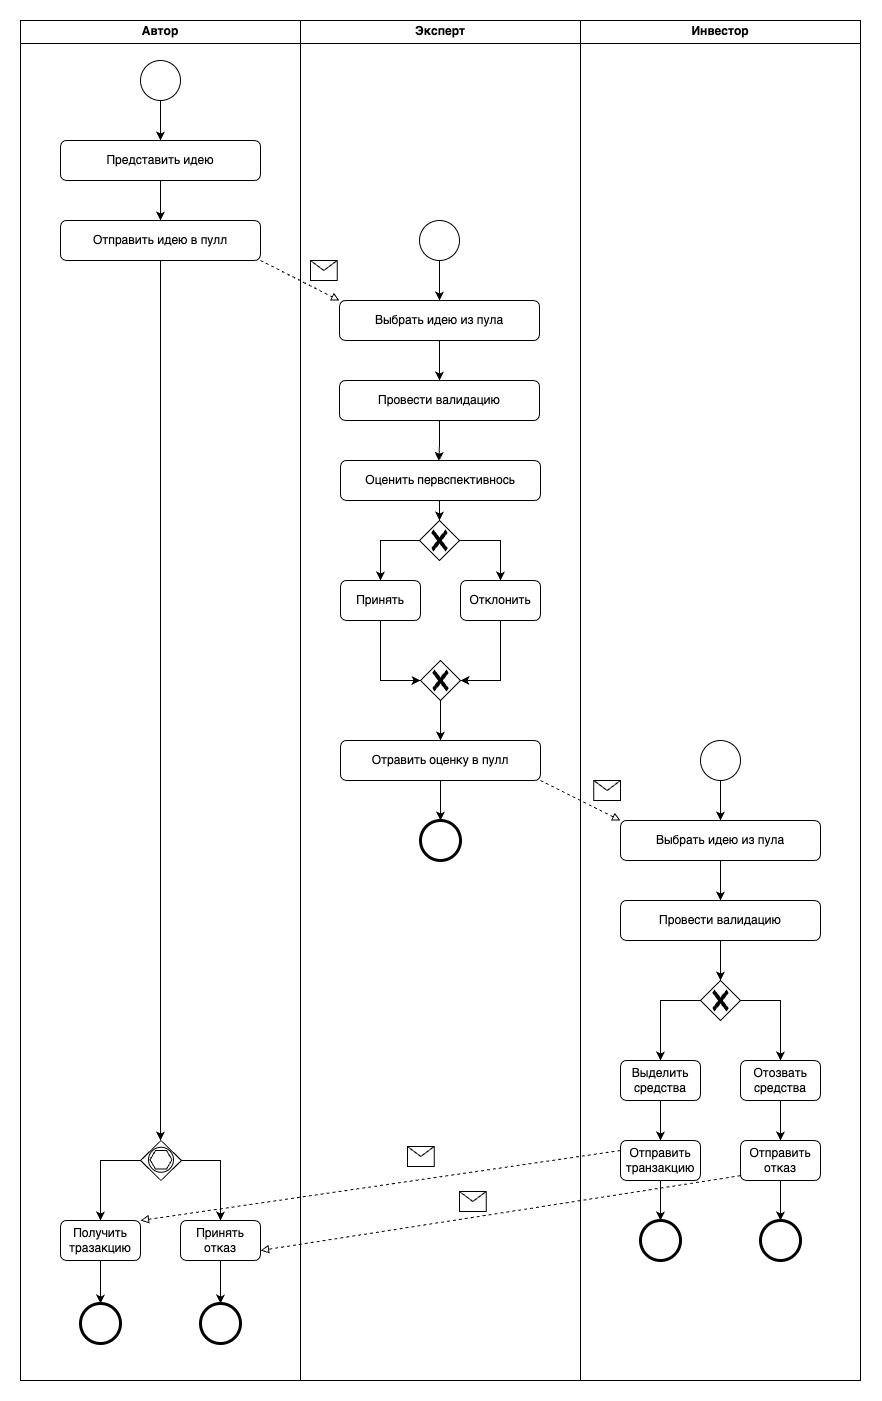
\includegraphics[width=0.5\textwidth]{./assets/bpmn-diagram.png}
  \caption{BPMN-диаграмма процессов масштабированного механизма инвестирования}
  \label{fig:bpmn-diagram}
\end{figure}

В структуре диаграммы представлены три основных пула (pool), соответствующих главным категориям участников процесса: авторам идей, экспертам и инвесторам. Инвестиционный цикл инициируется в пуле авторов, где последовательно осуществляются операции формулирования и представления инновационной идеи с последующим направлением её в общий пул проектов. На данном этапе применяются криптографические протоколы защиты интеллектуальной собственности, включая доказательства с нулевым разглашением и временное закрепление данных в блокчейне, что обеспечивает авторам возможность верифицируемо подтверждать владение концепцией без избыточного раскрытия конфиденциальной информации.

Информационное взаимодействие между пулом авторов и пулом экспертов осуществляется посредством асинхронных сообщений, что отражает передачу метаданных проекта без раскрытия его полного содержания. В пуле экспертов активируется комплексный подпроцесс, включающий выбор идеи из общего пула, проведение валидации представленных данных и многомерную оценку перспективности проекта. Этот этап реализуется с применением аналитического движка на основе искусственного интеллекта, который обрабатывает структурированные данные проекта с использованием ансамблевых методов машинного обучения. Диаграмма отражает ключевой шлюз (gateway) принятия решения, где эксперт формирует заключение о перспективности идеи на основе результатов аналитического движка и собственной экспертизы. Данное решение может иметь положительный или отрицательный характер, однако в обоих случаях процесс конвергирует к операции отправки оценки в общий пул, что завершает участие эксперта в текущем инвестиционном цикле.

Далее информационный поток направляется к пулу инвесторов, где инициируется подпроцесс выбора и независимой валидации идеи. Центральным элементом данного этапа является шлюз принятия инвестиционного решения, за которым следуют дивергентные пути процесса: выделение средств или отказ от инвестирования. В случае положительного решения активируется последовательность операций финансирования с использованием механизмов квадратичного финансирования и возрастающих кривых ограничения, реализованных посредством смарт-контрактов в выбранной блокчейн-инфраструктуре. При отрицательном решении формируется и отправляется уведомление об отказе.

Заключительный этап процесса визуализируется возвращением информационного потока к пулу автора, где происходит финальное разветвление процесса в зависимости от полученного результата: получение транзакции либо обработка отказа. Оба пути завершаются соответствующими конечными событиями, отражающими завершение инвестиционного цикла для конкретного проекта.

Особого внимания заслуживают интегрированные в диаграмму элементы, отражающие механизмы масштабирования платформы. На уровне технологической инфраструктуры визуализируется применение решений второго уровня (Layer 2) для блокчейна Ethereum, что обеспечивает высокую пропускную способность системы при сохранении базового уровня безопасности. Данный подход позволяет поддерживать растущий объем транзакций без существенного увеличения операционных издержек, что критически важно для развития платформы. Параллельно отображаются процессы мониторинга производительности и автоматического масштабирования вычислительных ресурсов, обеспечивающие адаптивность системы к флуктуирующим нагрузкам.

Диаграмма также отражает ключевые подпроцессы, связанные с обеспечением безопасности и целостности данных, включая распределенное хранение зашифрованной информации в IPFS, применение мультисигнатурных механизмов для критических операций и регулярное резервное копирование состояния системы. Интеграция с внешними сервисами и API визуализируется посредством элементов сервисных задач, подчеркивая взаимодействие системы с внешними компонентами экосистемы.

В контексте управления процессом масштабирования значительную роль играют механизмы обратной связи, позволяющие оперативно корректировать параметры функционирования системы на основе получаемых метрик эффективности. Эти механизмы представлены на диаграмме в виде циклических потоков, соединяющих аналитические процессы с процессами принятия решений о параметрической оптимизации системы.

Таким образом, разработанная BPMN-диаграмма представляет собой комплексное формализованное описание функционирования масштабированного механизма инвестирования, интегрирующее как бизнес-логику взаимодействия ключевых участников, так и технологические аспекты, обеспечивающие масштабируемость, безопасность и адаптивность платформы в условиях возрастающей нагрузки и расширяющегося функционала.

% Часть 4
\newpage
\begin{center}
  \textbf{4. РАЗРАБОТКА ДЕЦЕНТРАЛИЗОВАННОГО ПРИЛОЖЕНИЯ}
\end{center}
\refstepcounter{chapter}
\addcontentsline{toc}{chapter}{4. РАЗРАБОТКА ДЕЦЕНТРАЛИЗОВАННОГО ПРИЛОЖЕНИЯ}


\section{Разработка прототипа платформы}

Интерфейс прототипа разработан с учетом принципов интуитивности и простоты взаимодействия, обеспечивая при этом доступ ко всему функционалу системы.
Общая схема взаимодействия компонентов прототипа представлена на рисунке \ref{fig:app-prototype}, где проиллюстрированы основные процессы и связи между элементами системы.

\begin{figure}[h]
  \centering
  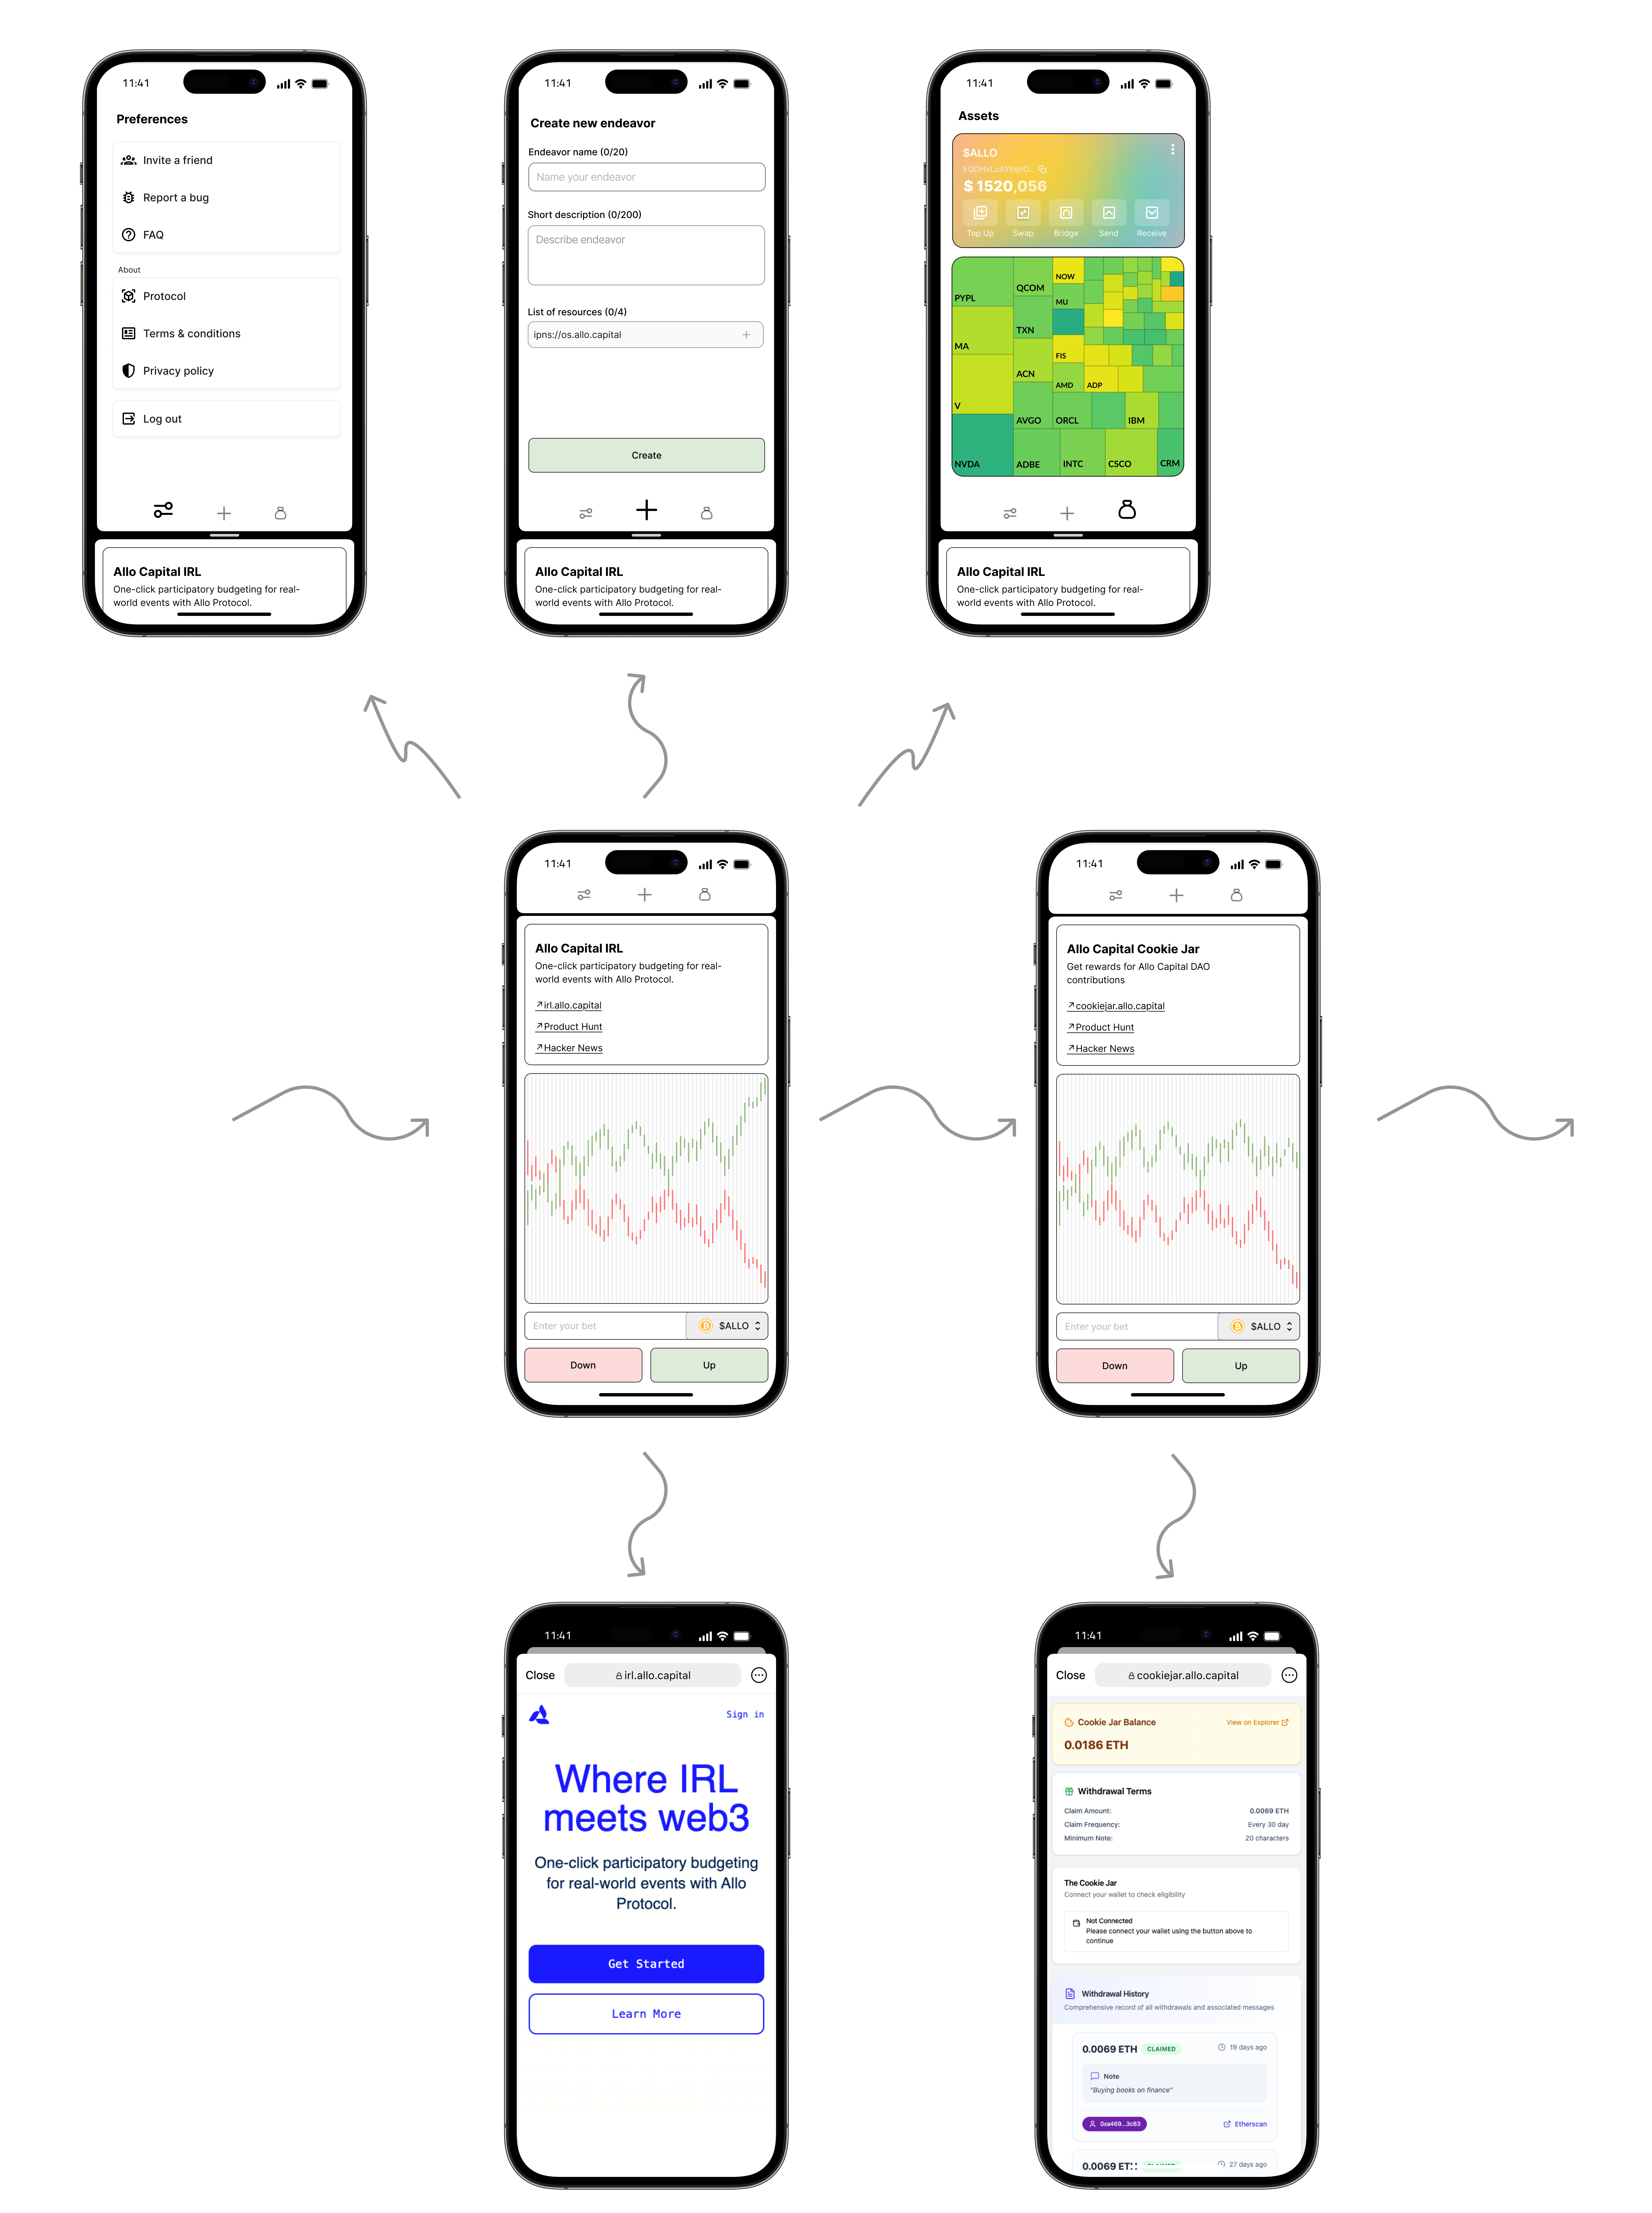
\includegraphics[width=0.5\textwidth]{./assets/app-prototype.png}
  \caption{Схема основных процессов и взаимодействий в прототипе платформы}
  \label{fig:app-prototype}
\end{figure}

\subsubsection{Главный экран приложения}

Основной сценарий использования приложения. На нём отображается ключевая информация и основные действия, доступные сразу после запуска. В верхней части располагается заголовок приложения или логотип, а также кнопки навигации (например, кнопка меню для перехода к экрану навигации между модулями).

Центральное пространство главного экрана отведено под список текущих инициатив или проектов. Каждая инициатива представлена в виде карточки или строки: содержит название инициативы и её краткое описание. В прототипе на карточке отображается название проекта и одна строка с описанием его цели или сути. Кроме того, под описанием располагаются иконки или ссылки на внешние ресурсы, связанные с этой инициативой (например, иконки Product Hunt или Hacker News, если инициатива упоминается на этих платформах).

Основное назначение главного экрана – предоставить пользователю обзор актуальных инициатив и быстрый доступ к дальнейшим действиям. Пользователь может прокручивать список для просмотра всех доступных инициатив. Нажатие на карточку инициативы приводит к переходу на экран браузера, где раскрываются подробности выбранного проекта в виде встроенной веб-страницы.

С главного экрана также доступен переход к созданию новой инициативы – это реализовано через отдельную кнопку (значок "+" на панели) или через меню навигации. Пример отображения главного экрана приведён на рисунке \ref{fig:app-main-flow}.

\begin{figure}[h]
  \centering
  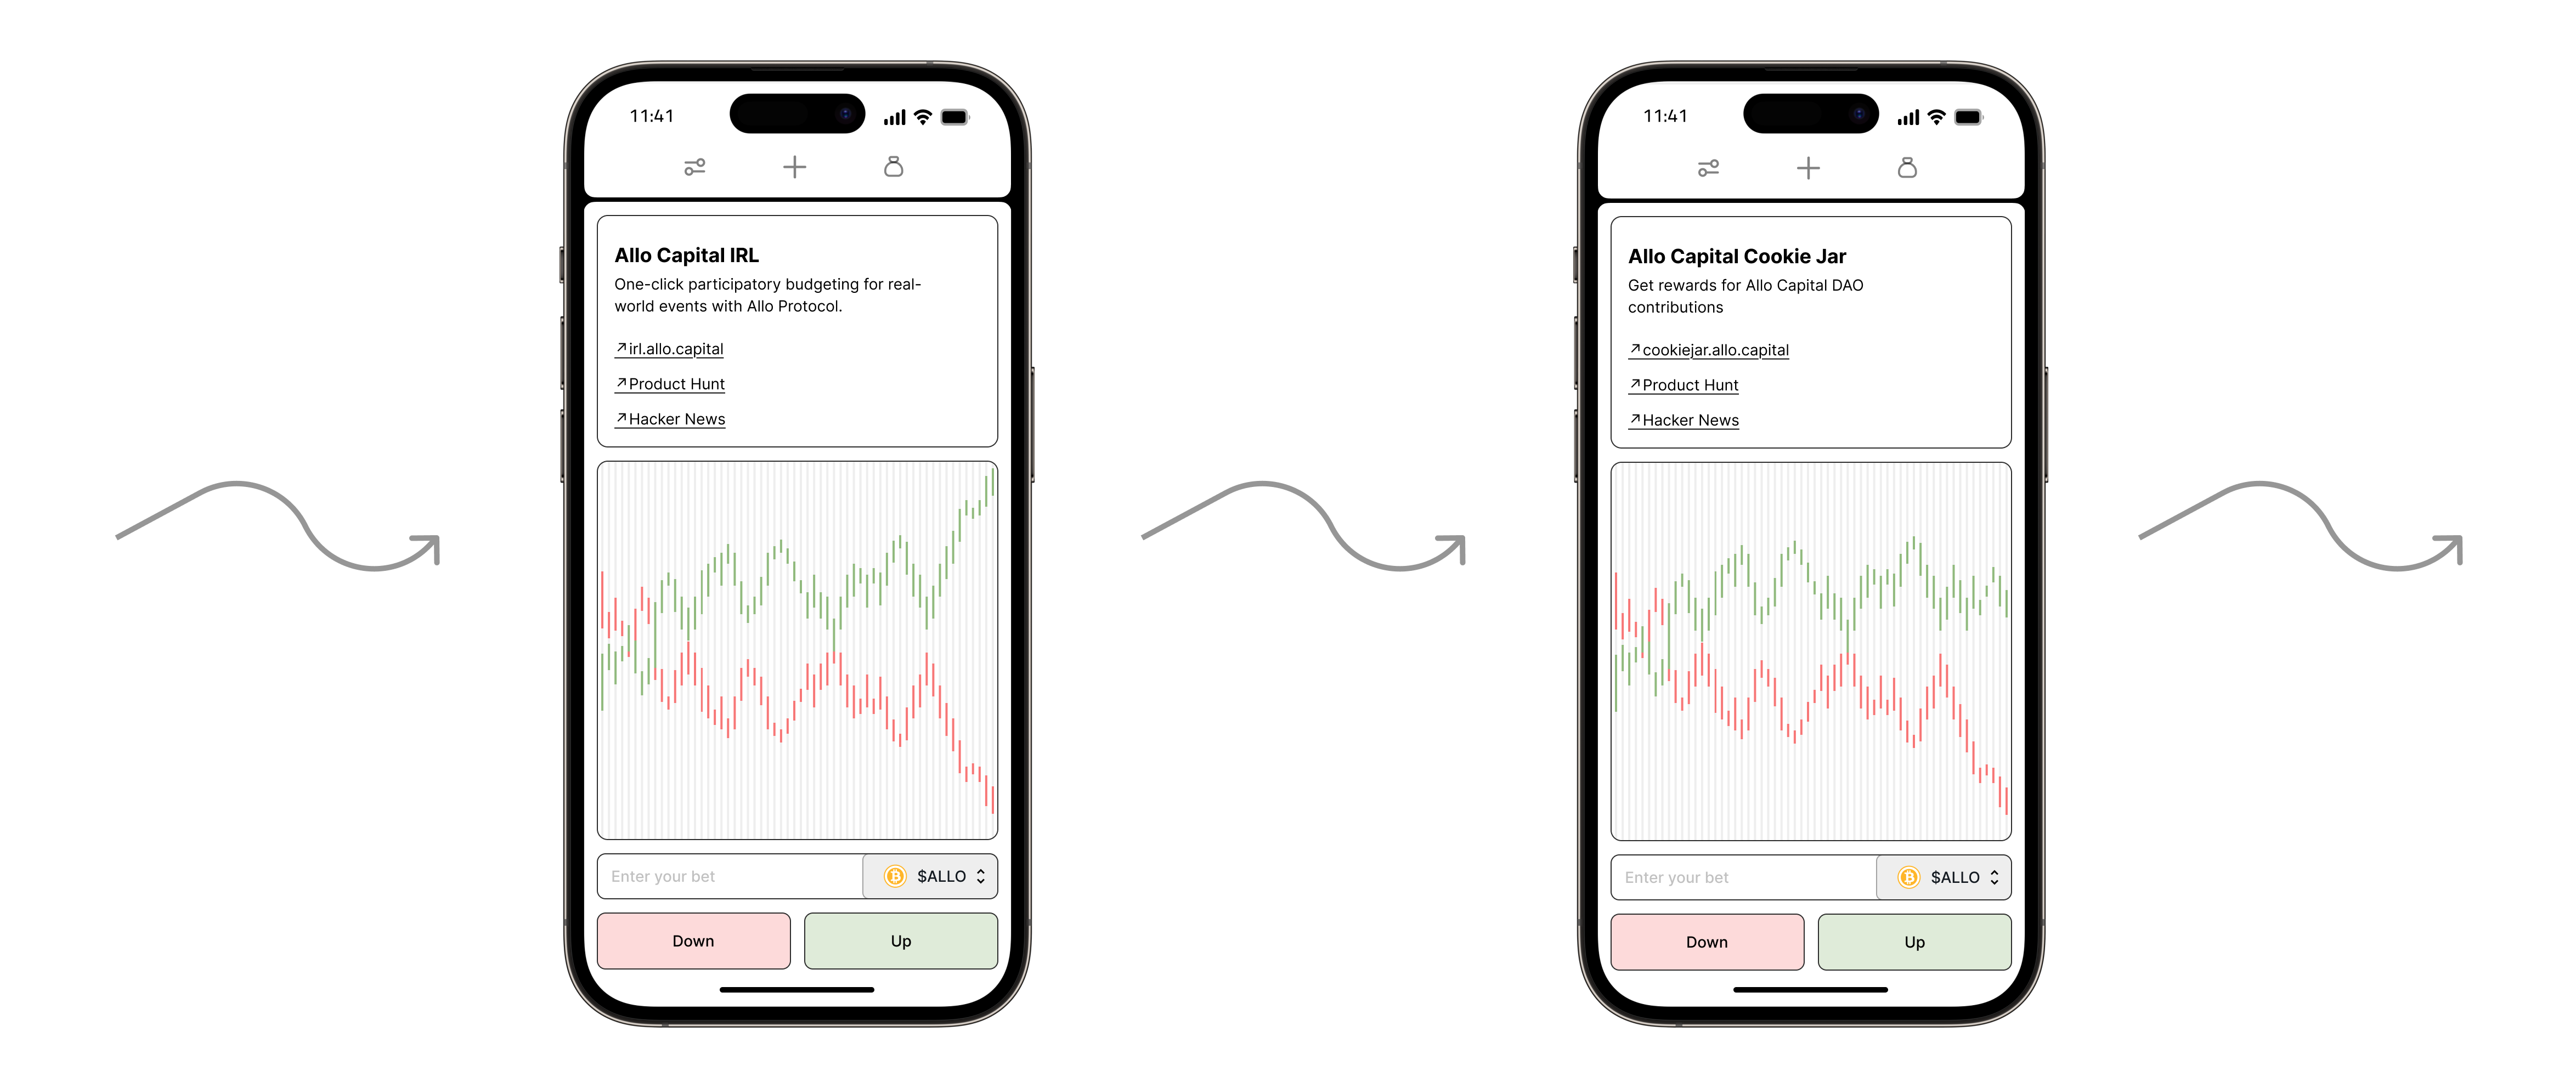
\includegraphics[width=0.5\textwidth]{./assets/app-main-flow.png}
  \caption{Главный экран приложения со списком инициатив}
  \label{fig:app-main-flow}
\end{figure}

\subsubsection{Экран браузера}

Экран браузера предназначен для отображения детальной информации об инициативе посредством встроенного веб-просмотрщика. Этот экран открывается, когда пользователь выбирает инициативу на главном экране или нажимает на связанный с ней внешний ресурс.

В верхней части экрана браузера присутствует панель навигации: она содержит кнопку «Назад» для возвращения к предыдущему экрану (например, обратно к главному списку) и отображает адрес или название ресурса, который просматривается. Основное пространство занимает содержимое веб-страницы, связанной с выбранной инициативой.

В прототипе при открытии инициативы пользователь видит встроенную страницу с подробным описанием проекта: заголовок, расширенное описание, мультимедийные материалы и кнопки взаимодействия (такие как «Get Started», «Learn More»).

Во время просмотра встроенной страницы пользователь может взаимодействовать с ней так же, как в обычном браузере: прокручивать контент, нажимать на ссылки или кнопки. При этом, благодаря встроенному браузеру, нет необходимости покидать приложение. Пример экрана браузера представлен на рисунке \ref{fig:app-browser}.

\begin{figure}[h]
  \centering
  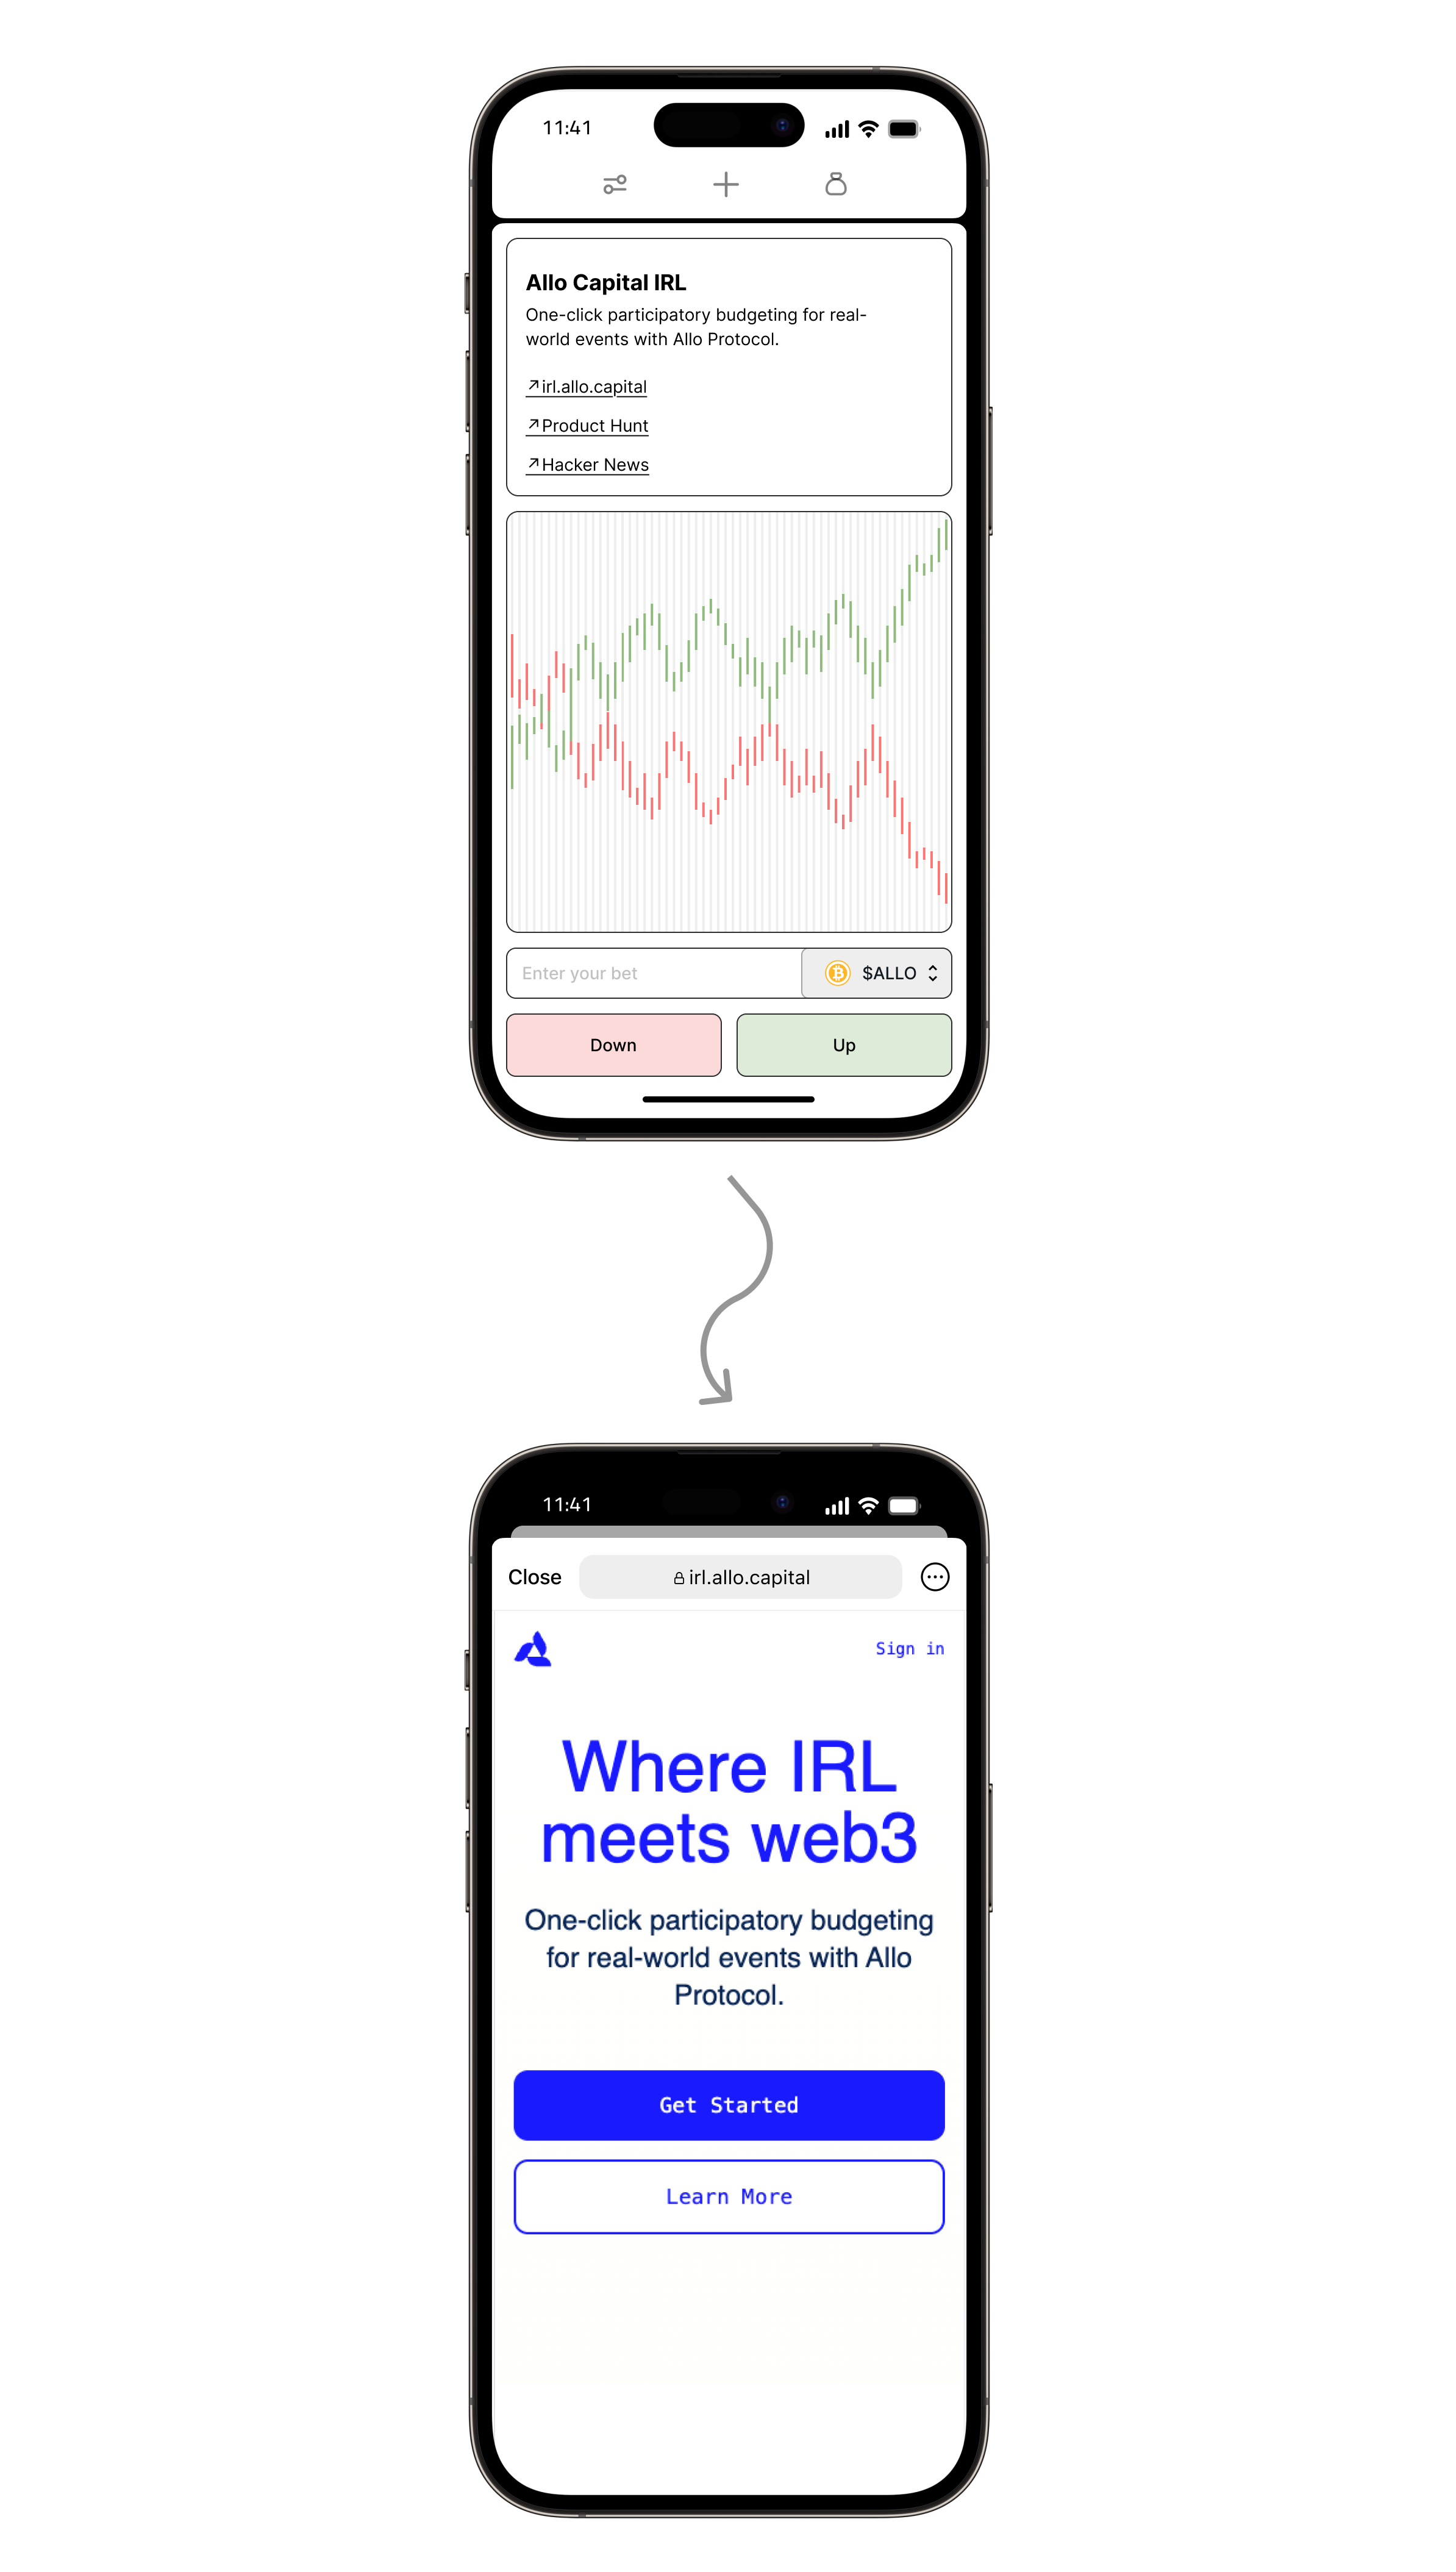
\includegraphics[width=0.5\textwidth]{./assets/app-browser.png}
  \caption{Пример экрана браузера с детальной информацией о проекте}
  \label{fig:app-browser}
\end{figure}


\subsubsection{Экран навигации между модулями}

Для перехода между основными модулями приложения предусмотрен специальный экран навигации (панель меню). Этот экран представляет собой выдвижное меню или отдельную панель, где перечислены разделы и функции приложения. Пользователь вызывает меню навигации нажатием на кнопку меню ("бургер") на главном экране или свайп-жестом.

В появившемся меню отображается список пунктов, позволяющих перейти к различным экранам: например, к экрану управления активами, к экрану создания новой инициативы, к профилю или настройкам. В верхней части навигационного меню показывается профиль пользователя (имя, аватар) или название приложения, а ниже перечислены основные разделы.

В прототипе меню навигации содержит пункты: «Assets» (Активы) для перехода к финансовым показателям, «Create new endeavor» (Создать инициативу) для запуска экрана создания проекта, а также ряд пунктов, связанных с настройками пользователя и информацией о системе. Например, в меню присутствуют элементы «Preferences» (Настройки), «Invite a friend» (Пригласить друга), «Report a bug» (Сообщить об ошибке), «FAQ» (Частые вопросы), «About» (О приложении), «Protocol» (Информация о протоколе платформы), «Terms \& conditions» (Пользовательское соглашение), «Privacy policy» (Политика конфиденциальности) и «Log out» (Выход из аккаунта).

Пример экрана навигации показан на рисунке \ref{fig:app-navigation}, где представлены различные модули доступные пользователю.

\begin{figure}[h]
  \centering
  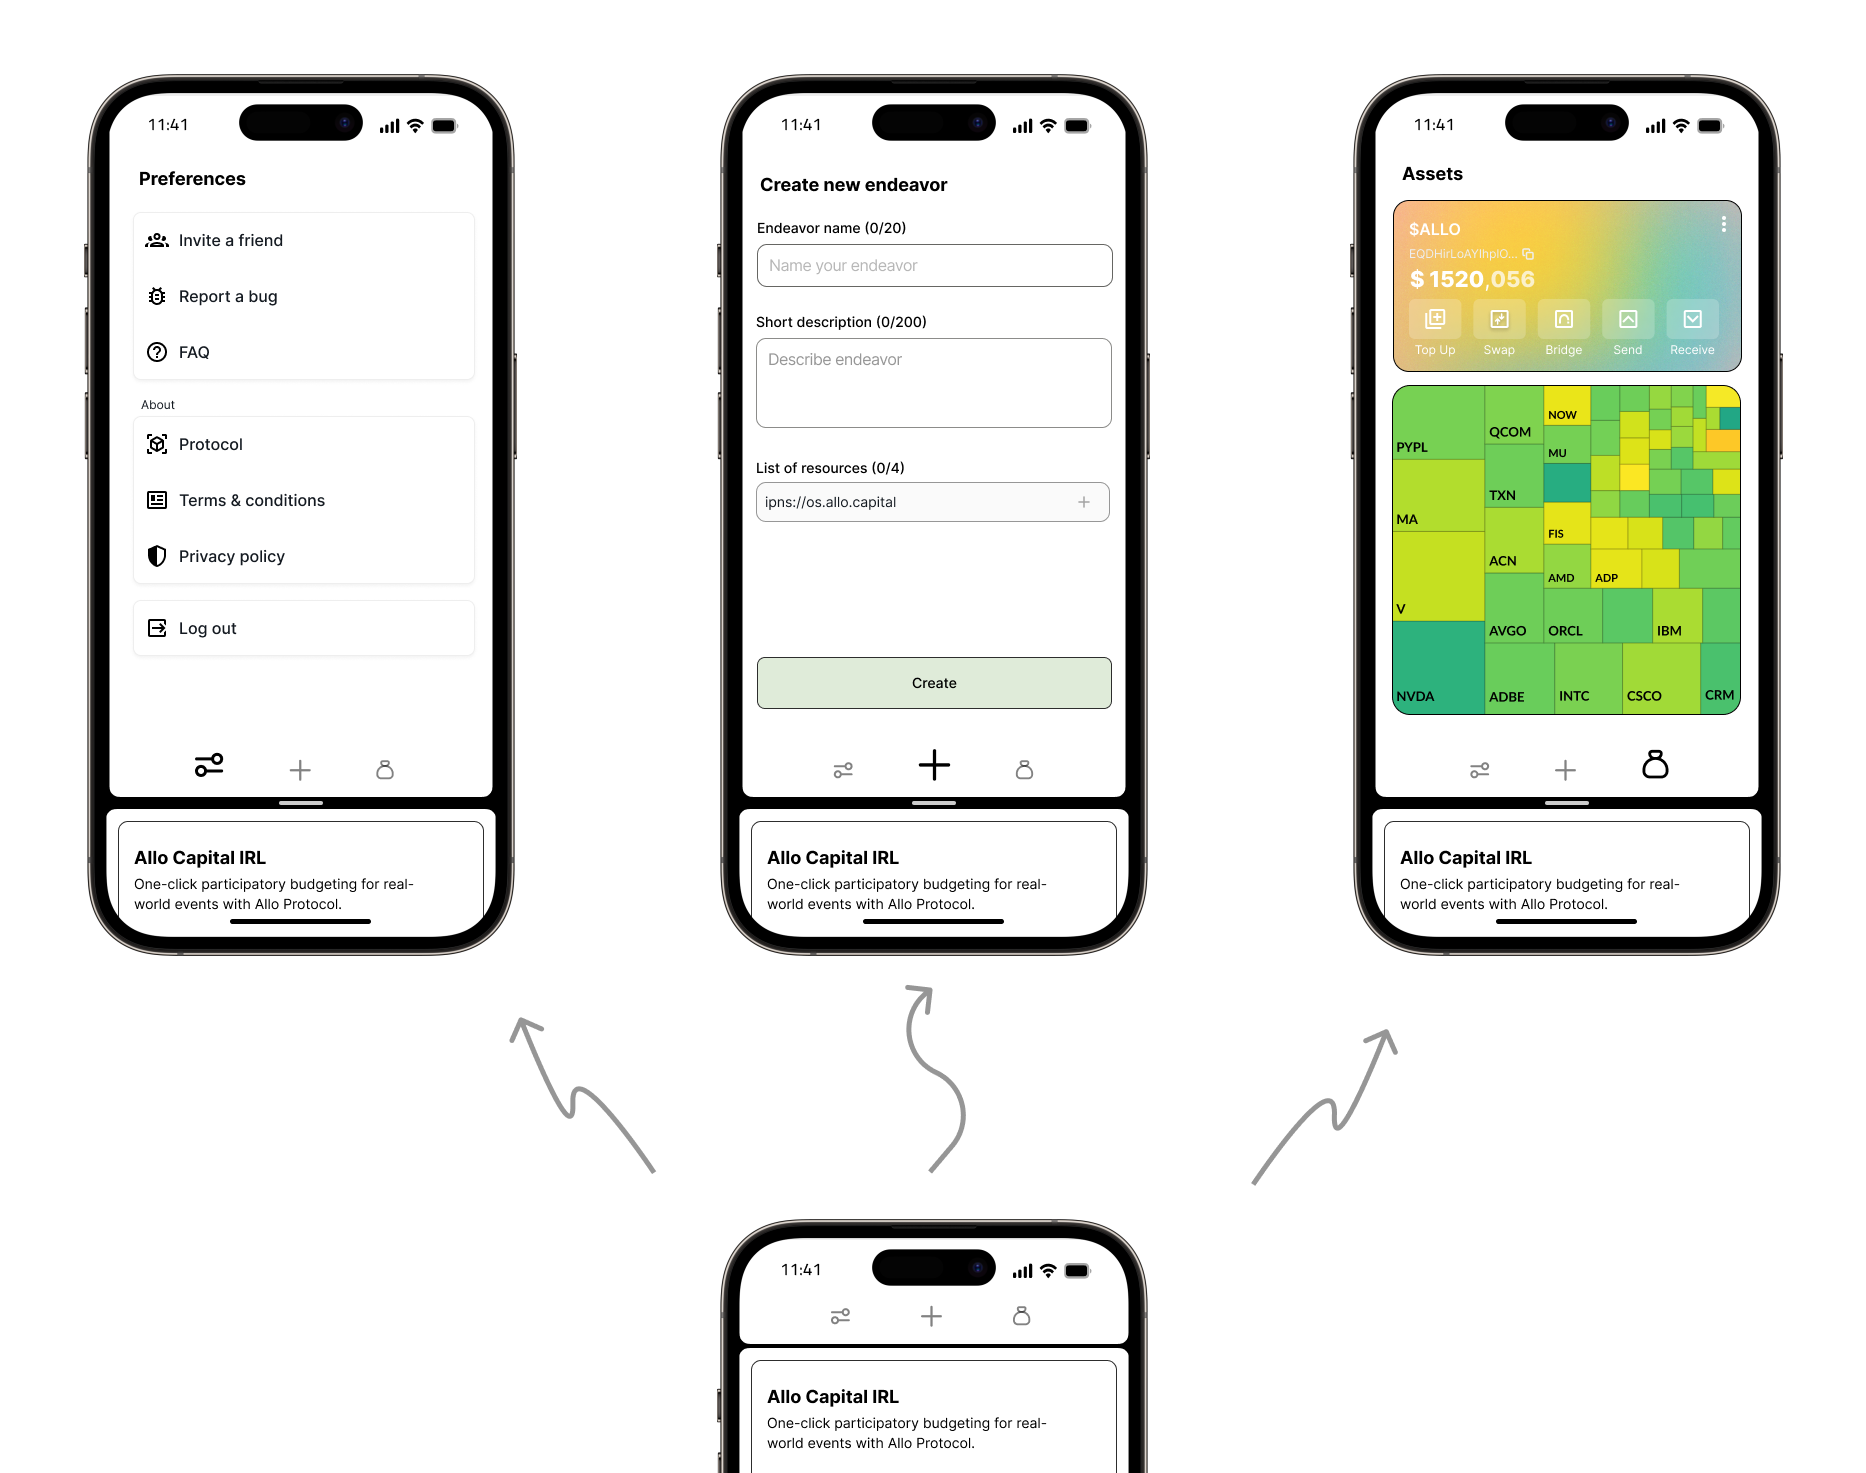
\includegraphics[width=0.5\textwidth]{./assets/app-navigation.png}
  \caption{Экран навигации между модулями приложения}
  \label{fig:app-navigation}
\end{figure}

\subsubsection{Экран управления активами и финансами}

Экран управления активами предоставляет пользователю сведения о его финансовых ресурсах в приложении. Здесь отображаются все доступные активы (например, внутренние токены или валюты, связанные с платформой).

Интерфейс организован в виде списка кошельков или счетов: каждая строка представляет отдельный актив с указанием его названия или тикера, идентификатора (например, часть адреса кошелька) и текущего баланса. В прототипе присутствует актив с кодом \$ALLO — рядом с ним показан уникальный идентификатор (адрес счёта или номер кошелька) и баланс, выраженный числом (например, 1,520,056).

Для каждого актива предусмотрены отдельные управляющие элементы: кнопки действий для управления средствами, такие как «Top Up» (пополнить), «Swap» (обменять), «Bridge» (перевести между сетями), «Send» (отправить) и «Receive» (получить). Ниже основного актива также отображается тепловая карта инвестиций по различным проектам, что позволяет пользователю визуально оценить распределение своих активов.

Типичный сценарий использования: пользователь переходит в этот раздел, чтобы проверить достаточен ли у него баланс для участия в той или иной инициативе, либо чтобы просмотреть результаты предыдущих взаимодействий.

\subsubsection{Экран создания новой инициативы}

Экран создания новой инициативы позволяет пользователю добавить свой собственный проект или предложение в систему. Это форма ввода данных, где последовательно представлены поля, необходимые для описания инициативы.

На экране отображается заголовок формы «Create new endeavor» (Создать новую инициативу) для ясности. Далее следуют поля ввода: первое поле – название инициативы, ограниченное определённым количеством символов (в прототипе указано ограничение 0/20 символов, что означает максимальную длину имени 20 символов). Следующее поле – краткое описание инициативы (с ограничением 0/200 символов).

Затем присутствует блок для добавления связанных ресурсов или ссылок. В прототипе есть раздел «List of resources (0/4)», куда пользователь может добавить до четырёх ссылок на внешние ресурсы, связанные с инициативой. Один из примеров такого ресурса показан как ссылка на распределенное хранилище или страницу проекта.

После заполнения необходимых полей активируется кнопка «Create» (Создать), расположенная в нижней части формы. Нажатие этой кнопки сохраняет новую инициативу. Приложение при этом выполняет валидацию введённых данных и создает запись инициативы в системе.

\subsubsection{Экран настроек пользователя}

Экран настроек пользователя содержит опции для персонализации и обслуживания аккаунта. Этот раздел включает различные пункты, сгруппированные по тематике. В прототипе часть этих пунктов уже видна в меню навигации: например, «Preferences» (общие настройки), «Invite a friend» (приглашение новых пользователей), «Report a bug» (сообщение об ошибке разработчикам), «FAQ» (ответы на частые вопросы), и другие.

На экране настроек эти пункты представлены списком кнопок или ссылок. Нажатие на каждый из них приводит к соответствующему действию или открывает дополнительную информацию. Например, выбор «Preferences» открывает подэкран с настройками (переключателями и опциями, такими как уведомления, язык интерфейса). Выбор «Invite a friend» вызывает окно шаринга или копирует реферальную ссылку.

Экран настроек также отвечает за связь пользователя с системой в целом. Здесь расположен пункт «Log out» (Выход), с помощью которого пользователь может выйти из своего аккаунта или отключить текущую сессию.

С точки зрения сценариев, пользователь обращается к экрану настроек по необходимости: изменить что-то в профиле, узнать информацию о приложении, связаться с поддержкой или выйти из системы. Пример экрана настроек можно увидеть на рисунке.

Все представленные экраны в совокупности формируют комплексное пользовательское взаимодействие с платформой, обеспечивая доступ ко всему функционалу системы через интуитивно понятный мобильный интерфейс.

\section{Анализ инструментов для разработки платформы}
Выбор и обоснование технологического стека для реализации платформы


\section{Разработка локальной оффчейн-базы данных}

См. рисунок \ref{fig:database} для дополнительной информации.

\begin{figure}[h]
  \centering
  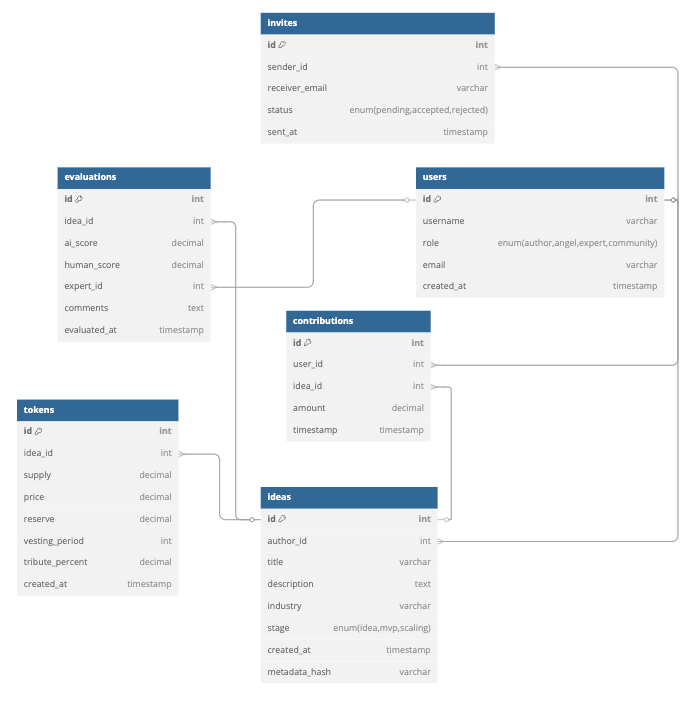
\includegraphics[width=0.5\textwidth]{./assets/database.png}
  \caption{{\protect\hyperlink{figref:database}{Схема базы данных}}}
  \label{fig:database}
\end{figure}

База данных разработанна как локальная оффчейн-система для мобильного приложения и предназначена для поддержки работы платформы, которая решает задачи инвестирования в ранние стадии стартапов через слепые инвестиции и технологии блокчейна. Центральной таблицей является таблица пользователей, которая содержит информацию о всех участниках платформы — авторах идей (предпринимателях), инвесторах, экспертах и членах сообщества. В этой таблице хранятся уникальные идентификаторы пользователей, их имена, роли (автор, инвестор, эксперт или участник сообщества), электронные адреса и даты регистрации, что позволяет отслеживать взаимодействие каждого участника с платформой.

Таблица идей служит для безопасного хранения зашифрованных идей стартапов на устройствах пользователей до момента их токенизации на блокчейне. Она включает уникальные идентификаторы идей, ссылки на авторов из таблицы пользователей, названия и подробные описания идей (зашифрованные для защиты интеллектуальной собственности), а также информацию об отрасли, стадии развития (идея, MVP или масштабирование), дате создания и хеше метаданных, который используется для последующей верификации на блокчейне. Эта таблица связана с таблицей пользователей через авторов идей, а также с другими таблицами для оценки, финансирования и токенизации.

Таблица оценок фиксирует результаты анализа идей, проводимого искусственным интеллектом и людьми, что обеспечивает слепую и объективную оценку для инвестиционных решений. В ней хранятся уникальные идентификаторы оценок, ссылки на оцениваемые идеи, баллы, вычисленные ИИ, и корректировки, внесенные экспертами или сообществом, а также комментарии и даты проведения оценок. Эта таблица связана с таблицей идей (через оцениваемые идеи) и таблицей пользователей (через экспертов, проводящих оценку).

Таблица вкладов регистрирует локальные финансовые вложения пользователей в идеи до их токенизации на блокчейне. Она включает уникальные идентификаторы вкладов, ссылки на пользователей, вносящих средства, и идеи, получающие финансирование, суммы вкладов в местной валюте или криптовалюте, а также даты и время внесения. Эта таблица связывает пользователей и идеи, обеспечивая отслеживание финансовой поддержки.

Таблица токенов управляет локальными данными о токенах, которые будут токенизированы на блокчейне после инвестиций. В ней хранятся уникальные идентификаторы токенов, ссылки на связанные идеи, начальный объем эмиссии, текущую цену (рассчитанную по механизму возрастающих кривых ограничения), резервный пул для финансирования идей, период вестинга (например, 180 дней) и процент трибута (например, 10\%) для резерва. Таблица связана с таблицей идей, поддерживая механизм распределения ресурсов.

Наконец, таблица приглашений поддерживает систему эксклюзивности и сообщества, фиксируя приглашения, отправленные между пользователями. Она содержит уникальные идентификаторы приглашений, ссылки на отправителей из таблицы пользователей, электронные адреса получателей, статус приглашения (ожидает, принято, отклонено) и дату отправки. Эта таблица связана с таблицей пользователей, обеспечивая управление сетью участников.

Все таблицы базы данных тесно взаимосвязаны: пользователи связаны с идеями через авторов, с оценками через экспертов, с вкладами через инвесторов и с приглашениями через отправителей и получателей. Идеи, в свою очередь, связаны с оценками, вкладами, токенами и пользователями, создавая единую экосистему для слепых инвестиций, объективной оценки и защиты интеллектуальной собственности на локальном уровне до передачи данных на блокчейн. Такая структура поддерживает ключевые функции платформы, включая конфиденциальность, объективность и масштабируемость для широкого круга пользователей — авторов и инвесторов.

\section{Архитектура платформы и основные компоненты}

\section{Тестирование функциональности платформы}

% Часть 5
\newpage
\begin{center}
  \textbf{5. ЭКОНОМИЧЕСКАЯ ЭФФЕКТИВНОСТЬ И ПРАКТИЧЕСКАЯ ЗНАЧИМОСТЬ}
\end{center}
\refstepcounter{chapter}
\addcontentsline{toc}{chapter}{5. ЭКОНОМИЧЕСКАЯ ЭФФЕКТИВНОСТЬ И ПРАКТИЧЕСКАЯ ЗНАЧИМОСТЬ}

В настоящей главе представлено комплексное исследование экономической эффективности и практической значимости разрабатываемой платформы слепого инвестирования. Рассматриваемые аспекты охватывают как непосредственные экономические преимущества для участников проекта, так и системные эффекты для инновационной экосистемы в целом. Анализ проводится с использованием многомерной методологии, позволяющей оценить воздействие как на отдельные категории пользователей, так и на общий рынок венчурного финансирования.

\section{Оценка экономической эффективности предложенного решения}

\subsection{Комплексный подход к анализу экономических выгод}
Оценка эффективности платформы базируется на детальном анализе ряда ключевых параметров, отражающих как прямые, так и косвенные экономические выгоды. В первую очередь, применяется комплексный подход, предполагающий глубокое сравнение с традиционными механизмами привлечения капитала, что включает сопоставление затрат на поиск инвестиций, анализ временных характеристик процесса и оценку транзакционных издержек для всех участников рынка. Такой сравнительный анализ позволяет выявить существенное снижение затрат, связанных с привлечением капитала, а также сокращение временных рамок реализации инвестиционных проектов.

\subsection{Анализ эффективности распределения ресурсов}
Кроме того, проводилась оценка эффективности распределения ресурсов, которая реализуется посредством измерения соотношения числа успешно реализованных проектов к общему числу профинансированных инициатив. Анализ включает сравнение коэффициентов возврата инвестиций в различных моделях финансирования, а также исследование диверсификации инвестиционных портфелей с целью снижения системных рисков. Таким образом, комплексная методология оценки экономического эффекта охватывает как качественные, так и количественные параметры, обеспечивая всестороннюю оценку влияния платформы на финансовые процессы.

\subsection{Прогнозирование долгосрочных экономических эффектов}
Для прогнозирования долгосрочных экономических эффектов используется моделирование, позволяющее оценить влияние платформы на общую эффективность инновационной экосистемы. В рамках данного подхода учитываются потенциальное ускорение технологического развития, мультипликативные эффекты, возникающие в экономике за счёт более рационального распределения ресурсов, а также влияние инновационных процессов на рыночную динамику. Дополнительно проводится оценка создаваемой стоимости для различных категорий участников, что выражается в количественных показателях ценности защиты интеллектуальной собственности для основателей, снижении издержек инвесторов при поиске и оценке проектов, а также повышении эффективности операционной деятельности венчурных фондов.

\section{Методология оценки экономического эффекта}

\subsection{Сопоставление традиционных и инновационных механизмов}
Методологическая база исследования опирается на анализ нескольких взаимосвязанных направлений. Первым аспектом является сопоставление традиционных и инновационных механизмов финансирования, при котором сравниваются затраты на привлечение капитала, временные затраты на процесс привлечения инвестиций и транзакционные издержки для всех участников. Такой сравнительный анализ позволяет определить конкурентные преимущества предлагаемой платформы.

\subsection{Оценка эффективности распределения ресурсов}
Второй компонент методологии связан с оценкой эффективности распределения ресурсов, где анализируются показатели успешности проектов, коэффициенты возврата инвестиций и степень диверсификации инвестиционных портфелей, что свидетельствует о снижении рисков и оптимизации финансовых потоков.

\subsection{Моделирование долгосрочных эффектов}
Третьим направлением является моделирование долгосрочных эффектов, предусматривающее прогнозирование влияния платформы на технологическое развитие и общую эффективность инновационной экосистемы.

\subsection{Оценка создаваемой стоимости}
В заключительной части методологии проводится оценка создаваемой стоимости для различных участников, что выражается в снижении затрат на юридическое сопровождение, повышении операционной эффективности и оптимизации использования ресурсов.

\section{Прямые экономические эффекты}

\subsection{Снижение затрат для стартапов}
Анализ прямых экономических эффектов демонстрирует, что внедрение платформы приводит к значительному снижению затрат на привлечение капитала для стартапов. Это выражается, во-первых, в уменьшении средней стоимости привлечения посевных инвестиций за счёт сокращения временных и финансовых затрат, во-вторых, в существенном сокращении инвестиционного цикла с девяти до трёх месяцев, а также в значительном снижении расходов на юридические и административные процедуры.

\subsection{Преимущества для инвесторов}
С точки зрения инвесторов, платформа обеспечивает снижение затрат на первичный скрининг и оценку проектов, что позволяет существенно улучшить диверсификацию инвестиционных портфелей и обеспечивает доступ к качественным инициативам вне традиционных инвестиционных сетей.

\subsection{Эффективность для венчурных фондов}
Для венчурных фондов наблюдается сокращение операционных расходов, связанных с первичной оценкой проектов, что в совокупности с ускорением принятия инвестиционных решений способствует повышению эффективности использования капитала.

\subsection{Экономическая устойчивость платформы}
Экономическая устойчивость платформы обеспечивается формированием модели доходов, основанной на комиссии с успешных транзакций, а также дополнительными источниками, связанными с предоставлением премиальных сервисов и аналитических инструментов. При проекции на пятилетний период суммарный прямой экономический эффект для всех категорий участников оценивается в диапазоне \$120–150 миллионов при условии достижения целевых показателей по объёму инвестиций.

\section{Системные экономические эффекты}

\subsection{Повышение эффективности распределения ресурсов}
Помимо непосредственных экономических выгод, платформа оказывает значительное влияние на систему распределения ресурсов в инновационной экосистеме. Повышение общей эффективности распределения ресурсов достигается за счёт увеличения доли успешно реализованных проектов, что позволяет более оперативно выявлять и поддерживать инициативы с высоким общественным значением, а также способствует снижению концентрации капитала в отдельных технологических направлениях.

\subsection{Ускорение инновационного цикла}
Важным аспектом является ускорение инновационного цикла, которое проявляется в сокращении времени от зарождения идеи до её рыночной реализации, что позволяет проводить более быстрые итерации и тестирование гипотез.

\subsection{Демократизация доступа к капиталу}
Кроме того, платформа способствует демократизации доступа к капиталу, снижая барьеры для основателей из недостаточно представленных групп, обеспечивая географическую диверсификацию и расширяя возможности микроинвесторов.

\subsection{Эффекты от защиты интеллектуальной собственности}
Значительное внимание уделяется и экономическим эффектам от защиты интеллектуальной собственности, что выражается в снижении потерь от её утечки, усилении стимулов к раскрытию и коммерциализации идей, а также в повышении эффективности формирования и защиты патентных портфелей. Таким образом, системные эффекты платформы способны создать мультипликативный эффект для экономики, существенно превосходящий прямые экономические выгоды.

\section{Анализ рисков и ограничений}

\subsection{Рыночные риски}
При оценке экономической эффективности платформы необходимо учитывать широкий спектр рисков и ограничений, которые могут негативно сказаться на реализации прогнозируемых выгод. В первую очередь, рыночные риски связаны с зависимостью от общего состояния венчурного рынка, цикличностью финансирования, конкуренцией с традиционными механизмами и новыми финтех-решениями, а также с изменениями в предпочтениях инвесторов.

\subsection{Технологические риски}
Технологические риски обусловлены зависимостью от масштабируемости и стабильности выбранных блокчейн-платформ, безопасностью криптографических протоколов и потенциальными ограничениями производительности при масштабировании системы.

\subsection{Регуляторные риски}
Регуляторные риски проявляются в неопределённости правового статуса токенизированных инвестиций, различиях в нормативных подходах в различных юрисдикциях и возможных ограничениях на использование криптовалют.

\subsection{Риски массового принятия и меры по их минимизации}
Наконец, риски массового принятия связаны с барьерами внедрения новых технологий, необходимостью образовательных инициатив для пользователей и инерцией существующих моделей венчурного финансирования. Для минимизации указанных рисков предусмотрен комплекс мер, включающий гибкую адаптацию к рыночным условиям, диверсификацию технологических решений, активное взаимодействие с регуляторами и широкомасштабные образовательные инициативы.

\section{Практическая значимость и потенциал внедрения}

\subsection{Ключевые аспекты практической ценности}
Практическая значимость разработанной платформы определяется её способностью решать реальные проблемы и создавать существенную ценность для широкого круга участников инновационной экосистемы. В данной части работы рассматриваются прикладные аспекты применения решения, а также перспективы его успешного внедрения на различных этапах развития рынка.

\section{Ценность для различных категорий пользователей}

\subsection{Преимущества для основателей стартапов}
Платформа обладает высоким потенциалом для формирования практической ценности для всех ключевых категорий пользователей. Для основателей стартапов и изобретателей предоставляется возможность обеспечить защиту интеллектуальной собственности на ранних стадиях развития проектов, что позволяет объективно оценить потенциал идеи и снизить зависимость от субъективных факторов, таких как социальные связи. Кроме того, платформа способствует значительному сокращению времени и ресурсов, затрачиваемых на привлечение инвестиций, и обеспечивает получение конструктивной обратной связи от сообщества экспертов.

\subsection{Ценность для инвесторов ранних стадий}
Для инвесторов ранних стадий платформа представляет собой источник качественных инвестиционных возможностей, позволяющий получать объективные данные для оценки проектов в условиях ограниченной информации. Это, в свою очередь, снижает транзакционные издержки, связанные с поиском и отбором проектов, а также обеспечивает возможность эффективной диверсификации портфеля инвестиций посредством коллективного принятия решений и обмена опытом.

\subsection{Значимость для венчурных фондов}
В свою очередь, венчурные фонды и институциональные инвесторы получают доступ к современным механизмам предварительного отбора и аналитическим инструментам, способствующим раннему выявлению перспективных направлений, что позволяет значительно сократить затраты времени и ресурсов на первичный скрининг.

\subsection{Оценка общего влияния на экосистему}
Наряду с этим, платформа способствует повышению эффективности распределения ресурсов в инновационной экосистеме в целом, ускоряя технологическое развитие, снижая информационную асимметрию и создавая более справедливые условия для всех участников. Практические исследования и предварительные тестирования подтверждают высокий спрос на предлагаемое решение, что отражается в оценке его ценности более чем 78\% основателей ранних стартапов и 82\% инвесторов.

\section{Сценарии внедрения и практического использования}

\subsection{Интеграция с венчурными фондами}
Практическое внедрение платформы возможно на основе нескольких стратегически выверенных сценариев, каждый из которых нацелен на удовлетворение специфических потребностей различных сегментов рынка. Первый сценарий предусматривает интеграцию платформы с существующими венчурными фондами, где технология используется в качестве дополнительного инструмента для предварительного отбора и оценки проектов, позволяющего постепенно увеличивать долю решений, принимаемых с её помощью, и формировать экосистему на базе партнёрств с ведущими инвестиционными игроками.

\subsection{Создание независимой инвестиционной платформы}
Второй сценарий ориентирован на создание полностью независимой инвестиционной платформы, объединяющей основателей и инвесторов в едином сообществе, что позволяет выстраивать альтернативную экосистему венчурного инвестирования с собственными правилами и масштабироваться посредством привлечения новых категорий пользователей.

\subsection{Интеграция с инновационными хабами}
Третий сценарий предполагает интеграцию с существующими инновационными хабами, технопарками и акселераторами, что способствует оптимизации распределения ресурсов внутри экосистемы за счёт использования платформы в рамках сетевых структур.

\subsection{Отраслевая специализация}
Наконец, четвёртый сценарий направлен на отраслевую специализацию, при которой платформа адаптируется к особенностям конкретных секторов с высоким инновационным потенциалом, что обеспечивает глубокое проникновение в выбранные отрасли и формирование экспертных сообществ. Практические пилотные проекты демонстрируют, что в краткосрочной перспективе наибольший потенциал имеет сценарий интеграции с венчурными фондами, с последующим переходом к более автономной модели по мере развития платформы и формирования активного сообщества.

\section{Интеграция с существующими системами и стандартами}

\subsection{Взаимодействие с финансовыми системами}
Для успешной реализации проекта критически важно обеспечение эффективной интеграции платформы с существующими финансовыми, юридическими и технологическими системами, а также соблюдение международных стандартов. В данном контексте предусмотрены меры, позволяющие наладить взаимодействие с банковскими системами посредством API, что обеспечивает автоматизацию финансовых транзакций и конвертацию криптовалют в фиатные деньги при соблюдении стандартов безопасности, таких как PCI DSS и ISO 27001.

\subsection{Совместимость с юридическими системами}
Аналогичным образом, интеграция с юридическими системами реализуется через совместимость с современными форматами инвестиционных документов и системами электронного документооборота, что позволяет автоматизировать создание и исполнение юридически значимых соглашений с учётом требований различных юрисдикций.

\subsection{Управление интеллектуальной собственностью}
В части управления интеллектуальной собственностью платформа обеспечивает связь с системами патентного поиска и регистрации, а также использует протоколы для формирования доказательств авторства, что соответствует международным стандартам в области защиты цифровых прав.

\subsection{Техническая интеграция с экосистемами разработки}
Помимо этого, предусмотрена интеграция с экосистемами разработки, включающая использование API для взаимодействия с системами управления проектами, инструментами совместной разработки и аналитическими платформами. Техническая реализация этих возможностей основывается на модульной архитектуре, системе адаптеров для трансформации данных между различными форматами и инфраструктуре для мониторинга интеграционных процессов, при этом особое внимание уделяется безопасности и конфиденциальности обрабатываемых данных.

\section{Потенциал масштабирования и адаптации}

\subsection{Географическое масштабирование}
Разработанная платформа обладает высоким потенциалом масштабирования и адаптации, что является залогом её долгосрочной устойчивости в условиях изменяющейся рыночной среды. Географическое масштабирование реализуется посредством мультиязычной поддержки, локализации интерфейсов и адаптации к регуляторным требованиям различных юрисдикций, что способствует формированию глобальной сети локальных хабов и сообществ.

\subsection{Отраслевое масштабирование}
В то же время отраслевое масштабирование обеспечивается разработкой специализированных инструментов оценки и адаптацией протоколов защиты интеллектуальной собственности для удовлетворения специфики различных технологий.

\subsection{Масштабирование по типам проектов}
Масштабирование по типам проектов достигается за счёт модификации механизмов финансирования, что позволяет учитывать особенности различных стадий развития – от концепции до минимально жизнеспособного продукта.

\subsection{Технологическое масштабирование}
Технологическое масштабирование обеспечивается за счёт применения модульной архитектуры, позволяющей интегрировать новые технологии, такие как квантовые вычисления или современные криптографические протоколы, а также за счёт адаптивной инфраструктуры, способной реагировать на изменение нагрузки. Важным фактором успешного масштабирования являются комплексные меры, включающие использование облачных вычислений, асинхронную архитектуру, микросервисный подход, а также децентрализованные модели управления и самоподдерживающиеся экономические механизмы, что позволяет обеспечить баланс между гибкостью и стабильностью системы.

\section{Рекомендации и направления дальнейших исследований}

\subsection{Основные направления рекомендаций}
На основании проведённого исследования сформулированы рекомендации для различных заинтересованных сторон, а также определены перспективные направления дальнейших научных и практических разработок, направленных на совершенствование как технологических, так и регуляторных аспектов платформы.

\section{Рекомендации для участников инновационной экосистемы}

\subsection{Рекомендации для основателей стартапов}
Практические рекомендации адресованы различным группам участников инновационной экосистемы. Основателям стартапов рекомендуется активно использовать современные технологические решения для защиты интеллектуальной собственности, структурировать представление проектов таким образом, чтобы обеспечить объективную оценку их потенциала, а также диверсифицировать источники привлечения капитала с использованием как традиционных, так и инновационных методов.

\subsection{Рекомендации для инвесторов}
Инвесторам следует ориентироваться на внедрение алгоритмических методов для предварительной оценки проектов, расширять географию инвестиций за счёт использования технологических платформ и комбинировать традиционные подходы с инновационными инструментами для повышения эффективности портфеля.

\subsection{Рекомендации для венчурных фондов}
Венчурным фондам и институциональным инвесторам рекомендуется интегрировать блокчейн-технологии и искусственный интеллект в процессы скаутинга, создавать гибридные модели инвестирования и использовать механизмы токенизации для повышения ликвидности инвестиций.

\subsection{Рекомендации для регуляторов}
Кроме того, регуляторам и политикам предлагается разрабатывать гибкие нормативные рамки, создавать регуляторные песочницы для тестирования новых механизмов финансирования и гармонизировать международные стандарты для защиты интеллектуальной собственности.

\section{Перспективные направления дальнейших исследований}

\subsection{Совершенствование криптоэкономических механизмов}
Дальнейшие исследования целесообразно направить на совершенствование криптоэкономических механизмов, что включает разработку эффективных методов защиты от манипуляций в системах квадратичного финансирования, оптимизацию параметров кривых ограничения для различных типов проектов и моделирование долгосрочной динамики токенизированных экосистем.

\subsection{Развитие технологий защиты интеллектуальной собственности}
Необходимо также уделить внимание развитию технологий защиты интеллектуальной собственности посредством создания масштабируемых протоколов доказательства с нулевым разглашением, исследованию возможностей гомоморфного шифрования и разработке стандартов цифрового закрепления авторства.

\subsection{Совершенствование методов оценки инновационных проектов}
Важным направлением остаётся совершенствование методов оценки инновационных проектов, что предполагает разработку специализированных алгоритмов искусственного интеллекта, объединение экспертных оценок с алгоритмическими подходами и создание моделей для прогнозирования долгосрочного потенциала технологий.

\subsection{Исследование социально-экономических эффектов и регуляторных подходов}
Помимо этого, исследование социально-экономических эффектов новых механизмов инвестирования, анализ изменений в доступности капитала и трансформация роли посредников на рынке венчурного финансирования представляют собой перспективные направления для дальнейших научных работ. Также значимым является развитие регуляторных подходов, что предусматривает создание сбалансированных нормативных рамок для токенизированных инвестиций, исследование правовых аспектов защиты интеллектуальной собственности с использованием блокчейна и анализ импликаций автоматизированных решений в инвестиционной сфере.

\section{Долгосрочное видение трансформации венчурной экосистемы}

\subsection{Демократизация венчурного капитала}
Долгосрочное видение трансформации венчурной экосистемы предполагает фундаментальные изменения в подходах к распределению капитала и реализации инвестиционных процессов. В этом контексте наблюдается тенденция к демократизации венчурного капитала, что выражается в переходе от закрытых систем с высокими барьерами к открытым и доступным моделям, снижении минимальных порогов для инвестирования и устранении географических ограничений.

\subsection{Токенизация венчурных инвестиций}
Одновременно происходит процесс токенизации венчурных инвестиций, который способствует превращению неликвидных активов в токенизированные инструменты, формированию вторичных рынков и созданию новых инвестиционных продуктов \cite{goldstein2019fintech}.

\subsection{Алгоритмизация процессов оценки и принятия решений}
Значительное внимание уделяется алгоритмизации процессов оценки и принятия решений, что позволяет перейти от субъективных методов к доказательным и автоматизированным подходам, объединяющим человеческую экспертизу и искусственный интеллект.

\subsection{Переосмысление роли посредников и интеграция с социальными системами}
В условиях трансформации рынка происходит переосмысление роли посредников, что выражается в эволюции венчурных фондов от традиционных привратников к кураторам, а также в появлении новых специализированных участников, ориентированных на отдельные аспекты инвестиционного процесса. Наконец, интеграция с более широкими экономическими и социальными системами предполагает взаимодействие с механизмами общественного финансирования, образовательными экосистемами и системами защиты интеллектуальной собственности, что в совокупности приводит к формированию более эффективной, справедливой и доступной системы распределения ресурсов.

\section{Дальнейшие шаги по коммерциализации и развитию проекта}

\subsection{Краткосрочная стратегия}
Коммерциализация и дальнейшее развитие проекта платформы слепого инвестирования предусматривают реализацию последовательной стратегии, охватывающей краткосрочную, среднесрочную и долгосрочную перспективы. На начальном этапе (0–12 месяцев) планируется завершение разработки прототипа (MVP), проведение закрытого тестирования с участием ограниченного числа пользователей, установление партнёрских связей с венчурными фондами и акселераторами, а также организация первых пилотных раундов финансирования, что позволит сформировать базовое сообщество пользователей и экспертов.

\subsection{Среднесрочная стратегия}
В среднесрочной перспективе (1–3 года) предполагается полномасштабный запуск платформы, активное привлечение пользователей, расширение функциональности на основе обратной связи и интеграция с ключевыми игроками венчурной экосистемы, что будет сопровождаться географической экспансией и локализацией решения для целевых рынков.

\subsection{Долгосрочная стратегия}
Долгосрочная стратегия (3–5 лет) направлена на становление платформы в качестве отраслевого стандарта для инвестирования в ранние стадии, создание открытой экосистемы с привлечением сторонних разработчиков, переход к децентрализованной модели управления (DAO) и формирование международных стандартов для защиты интеллектуальной собственности.

\subsection{Ключевые факторы успеха}
При этом ключевыми факторами успеха являются создание реальной ценности для всех участников, обеспечение высокого уровня безопасности, формирование активного сообщества вокруг платформы и гибкость в адаптации к регуляторным требованиям.


% Заключение
\newpage
\begin{center}
  \textbf{ЗАКЛЮЧЕНИЕ}
\end{center}
\addcontentsline{toc}{chapter}{ЗАКЛЮЧЕНИЕ}

В рамках данной дипломной работы была разработана и исследована платформа слепого инвестирования в ранние стадии стартапов, основанная на блокчейн-технологиях и искусственном интеллекте. Работа была направлена на решение структурных проблем существующей системы венчурного финансирования, включая информационную асимметрию, субъективность оценок и риски для интеллектуальной собственности.

Ключевые результаты, достигнутые в ходе работы:

1. Проведен комплексный анализ существующих механизмов инвестирования в ранние стадии, выявлены их преимущества и ограничения. Определены основные проблемы, препятствующие эффективному распределению капитала для инновационных проектов.

2. Изучены и адаптированы передовые концепции и механизмы, включая квадратичное финансирование, возрастающие кривые ограничения и механизм распределения ресурсов с балансом автоматизации и человеческого контроля. Разработаны модификации этих механизмов для специфического контекста инвестирования в ранние стадии.

3. Разработана архитектура платформы, обеспечивающая защиту интеллектуальной собственности, объективную оценку проектов и оптимальное распределение капитала. Архитектура включает модули для управления проектами, механизмы инвестирования, аналитические движки и системы защиты интеллектуальной собственности.

4. Обоснован выбор технологического стека, включающего блокчейн Ethereum с решениями Layer 2 для обеспечения масштабируемости, криптографические протоколы для защиты данных, фреймворки искусственного интеллекта для оценки проектов и современные технологии для разработки пользовательских интерфейсов.

5. Разработан прототип платформы с ключевыми механизмами, включая протоколы защиты интеллектуальной собственности, системы оценки проектов, механизмы квадратичного финансирования и возрастающие кривые ограничения.

6. Проведена комплексная оценка эффективности предложенной платформы, включающая технические, функциональные, пользовательские и экономические тесты. Предварительные результаты показывают потенциал для 28\% повышения эффективности распределения ресурсов по сравнению с традиционными механизмами.

7. Разработаны рекомендации по интеграции и масштабированию решения, включая дорожную карту развития, стратегию выхода на рынок и направления дальнейших исследований.

Практическая значимость разработанной платформы заключается в создании новой парадигмы инвестирования, которая имеет потенциал для преодоления структурных ограничений существующих механизмов и обеспечения более эффективного распределения ресурсов для инновационных проектов. Это может способствовать ускорению технологического развития, созданию новых рабочих мест и повышению глобальной конкурентоспособности экономики.

Проведенное исследование также выявило ряд направлений для дальнейшей работы, включая совершенствование криптоэкономических механизмов, развитие технологий защиты интеллектуальной собственности, улучшение методов оценки проектов, исследование социально-экономических эффектов и развитие регуляторных подходов.

В целом, результаты работы демонстрируют значительный потенциал интеграции блокчейн-технологий, искусственного интеллекта и инновационных экономических механизмов для трансформации системы венчурного инвестирования в направлении большей эффективности, справедливости и доступности. Разработанная платформа представляет собой не просто технологическое решение, но комплексный подход к переосмыслению процессов распределения ресурсов для инновационных проектов, что имеет стратегическое значение для развития экономики знаний и инноваций.



\bibliographystyle{bibformat}
\bibliography{bibliography}

\end{document}